\documentclass{Academic}

\begin{document}
%Easy customisation of title page
%TC:ignore
\myabstract{\small
\noindent\textbf{Abstract}
%Abstract below

This study presents a comparative evaluation of the Ad hoc On-Demand Distance Vector (AODV) and Optimized Link State Routing (OLSR) protocols in a Mobile Ad Hoc Network (MANET) using the NS-3 simulator. The purpose of the research is to examine how reactive and proactive routing strategies perform under the same simulation conditions and to determine their relative strengths across key network performance metrics. A repeatable simulation scenario was designed in NS-3, and FlowMonitor was used to extract quantitative results from multiple simulation runs. The analysis focuses on packet delivery ratio, throughput, end-to-end delay, jitter, and packet loss, as these metrics provide a direct basis for assessing routing effectiveness in dynamic wireless environments.

The study is motivated by the fact that MANET routing performance is highly dependent on scenario configuration, including mobility, traffic behaviour, and network scale, meaning that controlled comparative testing remains necessary. In addition to metric extraction and graphical visualisation, AI-assisted analysis was incorporated as a secondary interpretive layer to help identify trends, organise comparative observations, and strengthen the clarity of result discussion. The AI component was applied only after simulation outputs had been generated and did not modify the original measured data.

The contribution of the study lies in providing a structured and reproducible workflow for comparing AODV and OLSR using NS-3 and FlowMonitor while also demonstrating a careful and transparent use of AI in simulation-based network analysis. The research therefore combines protocol comparison, repeatable experimentation, and assisted interpretation in a form intended to reflect both technical implementation and academic research rigour.
}
\renewcommand{\myTitle}{Performance Evaluation of AODV and OLSR Routing Protocols in NS-3 with AI-Assisted Analysis}
\renewcommand{\MyAuthor}{Anthony Edjenuwa}
\renewcommand{\MyDepartment}{Systems \& Security Engineer | Founder, ArxNova Networks }
\renewcommand{\ID}{info@edjenuwa.tech}
\renewcommand{\Keywords}{MANET, NS-3, AODV, OLSR, FlowMonitor, routing protocols, performance evaluation, packet delivery ratio, throughput, delay, jitter, packet loss, AI-assisted analysis}
\maketitle
%\vspace{-1.9em}\noindent\rule{\textwidth}{1pt} %add this line if not using abstract
\onehalfspacing
%TC:endignore

\section{Introduction}

Mobile Ad Hoc Networks (MANETs) are infrastructure-less wireless networks in which mobile nodes communicate through self-organised multi-hop routing rather than fixed network equipment. Their flexibility makes them relevant to scenarios such as emergency response, military communication, temporary deployments, and other dynamic environments where rapid network formation is required \parencite{boukerche2009,loo2016,sarkar2016}. However, the absence of centralised control and the presence of node mobility make routing a fundamental challenge in MANET design, since communication paths can change frequently and unpredictably \parencite{perkins2003aodv,clausen2003olsr,patel2015}.

Among the most widely studied MANET routing protocols are Ad hoc On-Demand Distance Vector (AODV) and Optimized Link State Routing (OLSR). AODV is a reactive protocol that establishes routes only when needed, whereas OLSR is a proactive protocol that maintains route information continuously through periodic control exchange \parencite{perkins2003aodv,clausen2003olsr}. This difference in routing strategy creates an important basis for comparison, since protocol behaviour can vary significantly depending on mobility, traffic load, and network scale \parencite{radha2018,kurniawan2020,sarkar2025}.

Although AODV and OLSR have been compared extensively in previous studies, performance findings often remain scenario-dependent. Differences in node density, terrain size, mobility models, and traffic patterns can lead to different conclusions about which protocol performs better \parencite{spaho2013,sallam2015,sallum2018,wang2022,kour2025}. This means there is still value in conducting controlled, repeatable experiments under clearly stated conditions, especially when the full workflow from simulation to analysis is made explicit.

This study therefore compares AODV and OLSR in NS-3 using FlowMonitor-based measurements obtained from repeated simulation runs. The analysis focuses on packet delivery ratio, throughput, end-to-end delay, jitter, and packet loss, since these metrics provide a direct basis for evaluating routing effectiveness in dynamic wireless environments \parencite{carneiro2009flowmonitor,riley2010ns3,selim2025}. In addition, AI-assisted interpretation is incorporated as a secondary analytical layer to support trend identification and improve the clarity of the discussion. The AI component is used only to assist analysis after metric extraction and does not replace the original simulation evidence \parencite{bhatia2022,duong2024,schuler2021}.

The study is motivated by three main factors. First, it seeks to provide a fair comparison between reactive and proactive MANET routing under a controlled NS-3 scenario. Second, it aims to demonstrate a reproducible workflow that combines simulation, FlowMonitor extraction, and graphical analysis. Third, it explores how AI-assisted interpretation can support simulation-based network research without compromising methodological transparency. On this basis, the research asks how AODV and OLSR differ under the configured scenario, which protocol performs better across the selected metrics, and how AI-assisted analysis contributes to the interpretation of results.

The main contribution of the work is a structured comparative evaluation of AODV and OLSR supported by a transparent experimental process and carefully bounded AI-assisted analysis. In this way, the project is positioned not only as a protocol comparison, but also as a demonstration of research rigour in simulation-based MANET performance evaluation.

\section{Background}

This section presents the conceptual basis of the study. It introduces Mobile Ad Hoc Networks (MANETs), outlines the main routing challenges they present, explains the distinction between reactive and proactive routing, and summarises the relevance of AODV, OLSR, NS-3, FlowMonitor, and AI-assisted analysis to the present research. The purpose of the section is to establish the theoretical foundation for the comparative methodology adopted later in the paper.

\subsection{Overview of Mobile Ad Hoc Networks}

Mobile Ad Hoc Networks (MANETs) are decentralised wireless networks in which mobile nodes communicate without fixed infrastructure or centralised administration. Nodes may function both as end devices and as intermediate routers, allowing communication to take place over multi-hop wireless paths when direct transmission is not possible \parencite{boukerche2009,loo2016,sarkar2016}. This makes MANETs relevant to dynamic environments such as emergency response, temporary deployments, and mobile field communication, where rapid and flexible network formation is required \parencite{patel2015,sarkar2025}.

\subsection{Routing Challenges in MANETs}

Routing in MANETs is difficult because the topology changes as nodes move, wireless links vary in quality, and the communication medium is shared. Under these conditions, routes may fail unexpectedly, while routing control traffic competes with application traffic for limited bandwidth \parencite{perkins2003aodv,clausen2003olsr,mohapatra2012}. As a result, MANET routing performance is commonly assessed using metrics such as packet delivery ratio, throughput, delay, jitter, and packet loss, since these reflect both reliability and transmission efficiency \parencite{sarao2022,selim2025,kour2025}.

\subsection{Routing Approaches in MANETs}

MANET routing protocols are commonly grouped into proactive, reactive, and hybrid approaches. Proactive protocols maintain routing information continuously, which improves route availability but increases control overhead. Reactive protocols create routes only when required, which can reduce unnecessary control exchange but may introduce route discovery delay \parencite{patel2015,loo2016,sarkar2016}. This distinction provides the conceptual basis for comparing OLSR and AODV in the present study.

\begin{figure}[H]
\centering
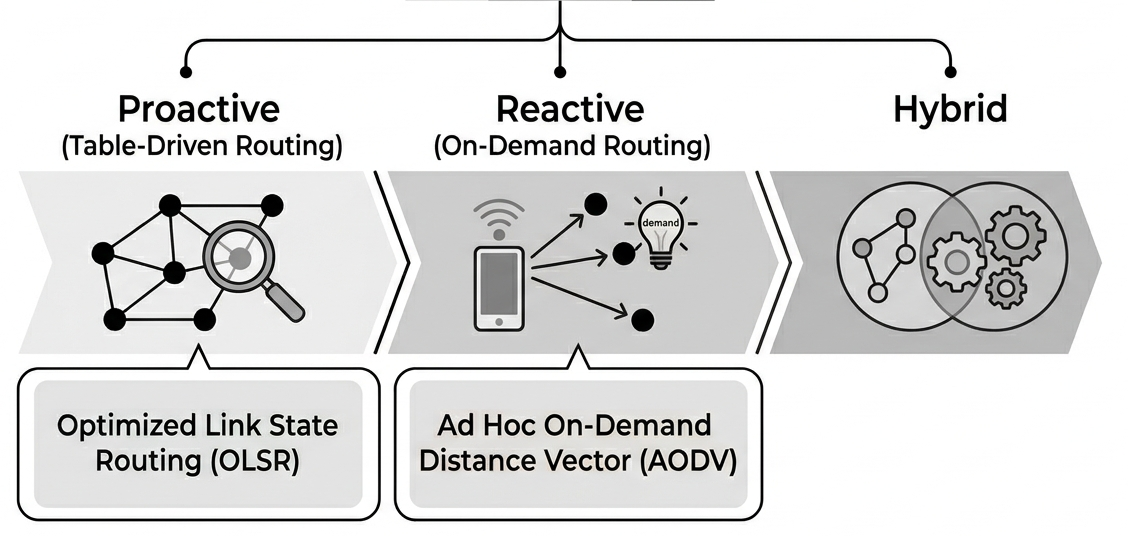
\includegraphics[width=0.70\textwidth]{figures/classification of Manet Protocol.png}
\caption{Classification of MANET routing protocols and the position of AODV and OLSR within reactive and proactive routing approaches.}
\label{fig:manet-classification}
\end{figure}

\subsection{Ad hoc On-Demand Distance Vector (AODV)}

AODV is a reactive routing protocol in which routes are established only when needed. When a source node has no valid route to a destination, it initiates route discovery through Route Request (RREQ) messages, while Route Reply (RREP) messages are used to return valid route information. Route Error (RERR) messages are then used to signal route failure when a link breaks \parencite{perkins2003aodv,belding2003,chakeres2004}. The protocol uses sequence numbers to preserve route freshness and reduce routing loops.

The main strength of AODV lies in its on-demand behaviour, since routes are not maintained unnecessarily when communication is inactive. However, this advantage may be offset by the delay introduced during route discovery and recovery, especially in highly dynamic topologies \parencite{midha2013,bappalige2020}. Figure~\ref{fig:aodv-discovery} illustrates the basic AODV route discovery and maintenance process.

\begin{figure}[H]
\centering
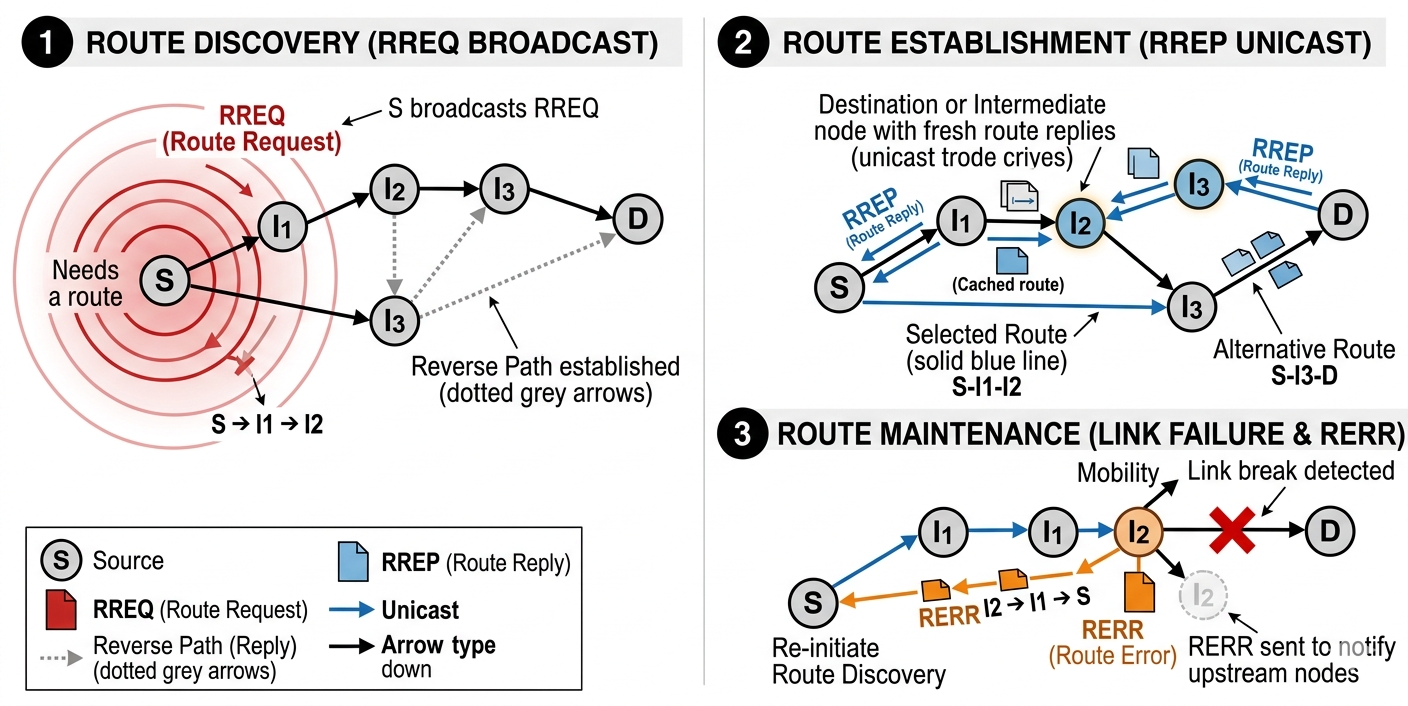
\includegraphics[width=0.78\textwidth]{figures/aodv route discovery process.png}
\caption{Simplified AODV route discovery and maintenance process.}
\label{fig:aodv-discovery}
\end{figure}

\subsection{Optimized Link State Routing (OLSR)}

OLSR is a proactive routing protocol that maintains routing information continuously through periodic exchange of control messages. A central feature of OLSR is the use of Multipoint Relays (MPRs), which reduce redundant flooding by allowing only selected nodes to retransmit topology information \parencite{clausen2003olsr,clausen2011nhdp,clausen2014olsrv2}. This mechanism improves dissemination efficiency while maintaining route awareness throughout the network.

The principal benefit of OLSR is route availability, since paths are already known when traffic begins. This can reduce forwarding delay compared with on-demand approaches, although it also introduces continuous routing overhead due to periodic updates \parencite{spaho2013,wheeb2023,sarkar2025}. Figure~\ref{fig:olsr-mpr} illustrates the role of control messaging and MPR selection in OLSR operation.

\begin{figure}[H]
\centering
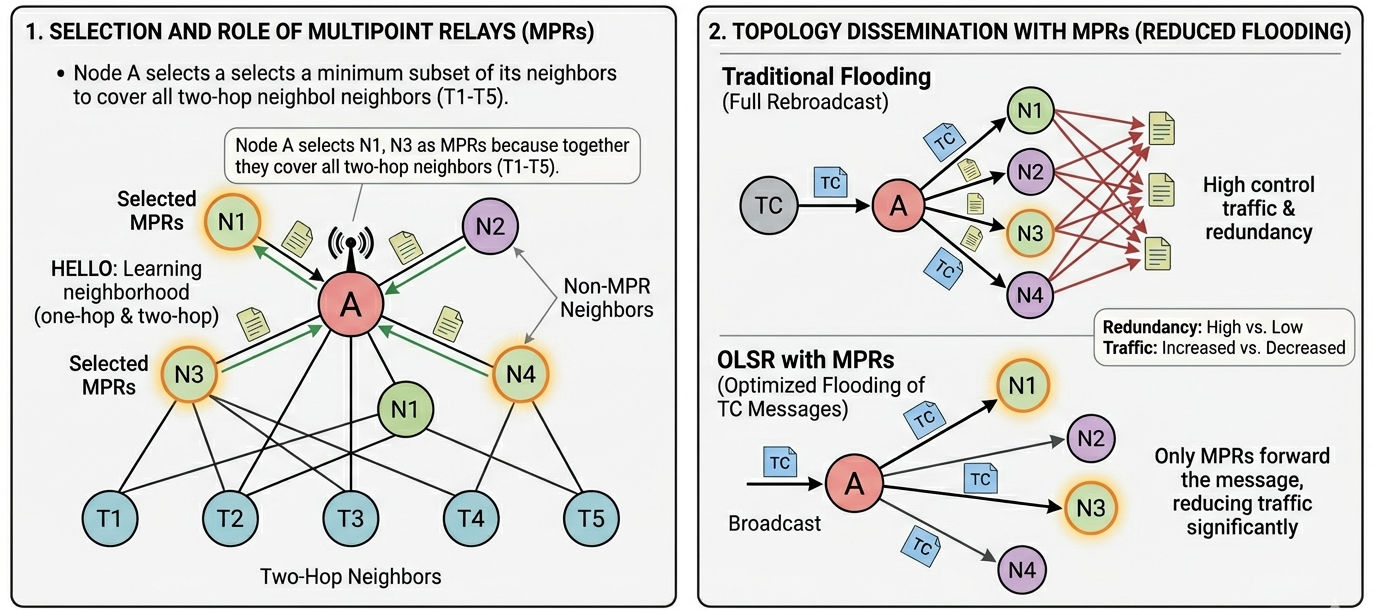
\includegraphics[width=0.78\textwidth]{figures/Olsr control and MPR diagram.png}
\caption{Simplified OLSR topology dissemination using Multipoint Relays (MPRs).}
\label{fig:olsr-mpr}
\end{figure}

\subsection{NS-3, FlowMonitor, and AI-Assisted Analysis}

NS-3 provides a controlled environment for repeatable routing experiments, while FlowMonitor supports structured extraction of flow-level statistics such as throughput, delay, jitter, and packet loss \parencite{riley2010ns3,carneiro2009flowmonitor,ns3flowmonitordocs}. In this study, these tools form the measurement framework for comparing AODV and OLSR under identical simulation conditions. AI-assisted analysis is then used only after metric extraction to support interpretation of patterns and comparative findings, without replacing the simulation evidence itself \parencite{bhatia2022,duong2024,schuler2021}.

\subsection{Section Summary}

This section has established the background of the study by outlining the nature of MANETs, the routing challenges they introduce, the distinction between reactive and proactive routing, and the operational principles of AODV and OLSR. It has also identified NS-3, FlowMonitor, and AI-assisted analysis as the main technical foundations of the research. These concepts provide the basis for the methodology and comparative evaluation presented in the next section.

\section{Methodology}

This section describes the methodology adopted for the comparative evaluation of AODV and OLSR in a MANET environment using NS-3. The study follows a quantitative, simulation-based design in which both routing protocols are evaluated under identical scenario conditions and measured using FlowMonitor-derived metrics. The methodology covers the design of the simulation scenario, protocol configuration, repeated execution of simulation runs, extraction of performance metrics, graphical analysis, and AI-assisted interpretation of results. The overall research workflow is presented in Figure~\ref{fig:methodology}.

\begin{figure}[H]
\centering
\begin{tikzpicture}[
    node distance=1.1cm and 1.2cm,
    stage/.style={
        align=center,
        text width=3.8cm,
        font=\bfseries\small
    },
    desc/.style={
        draw,
        rounded corners=6pt,
        fill=gray!10,
        align=center,
        text width=6.6cm,
        minimum height=1.1cm,
        font=\small
    },
    arrow/.style={->, thick}
]

\node[stage] (lit) {Literature Review\\and Research Framing};
\node[desc, right=of lit] (litd) {Review of MANET routing concepts, AODV, OLSR, NS-3, FlowMonitor, and formulation of the study aim and research questions.};

\node[stage, below=of lit] (design) {Simulation Scenario\\and Protocol Configuration};
\node[desc, right=of design] (designd) {Development of the 20-node MANET scenario in a $300 \times 300$ m area using Random Waypoint mobility and identical configuration of AODV and OLSR.};

\node[stage, below=of design] (exec) {NS-3 Execution\\and FlowMonitor Data Collection};
\node[desc, right=of exec] (execd) {Repeated execution of the simulation for both protocols and collection of flow-level statistics using FlowMonitor.};

\node[stage, below=of exec] (analysis) {Python-Based Metric Analysis\\and Visualisation};
\node[desc, right=of analysis] (analysisd) {Parsing of simulation outputs and computation of throughput, packet delivery ratio, delay, jitter, and packet loss, followed by graphical presentation.};

\node[stage, below=of analysis] (ai) {AI-Assisted Interpretation\\and Comparative Evaluation};
\node[desc, right=of ai] (aid) {Use of AI to support pattern identification and structured interpretation of results before the final protocol comparison.};

\draw[arrow] (lit) -- (design);
\draw[arrow] (design) -- (exec);
\draw[arrow] (exec) -- (analysis);
\draw[arrow] (analysis) -- (ai);

\end{tikzpicture}
\caption{Research methodology for the comparative evaluation of AODV and OLSR in NS-3 (research workflow presentation adapted from \parencite{golightly2023}.}
\label{fig:methodology}
\end{figure}

\subsection{Research Design}

This study adopts a quantitative, simulation-based comparative research design. The purpose of the research is to evaluate the performance of AODV and OLSR under the same MANET conditions so that any observed differences can be attributed primarily to the routing protocol rather than to changes in the simulation environment. This design is appropriate because the work focuses on measuring and comparing protocol behaviour across selected network performance metrics rather than proposing a new routing algorithm \parencite{riley2010ns3,carneiro2009flowmonitor,selim2025}.

The study is experimental in structure because the simulation parameters, mobility configuration, traffic generation, and data collection process are explicitly controlled. Both protocols are executed separately under identical settings, and the resulting outputs are collected through the same monitoring framework. This supports fairness, consistency, and reproducibility in the comparison process \parencite{campanile2020,ns3tutorial,manetcompare}.

\subsection{Experimental Environment and Tools}

The simulation environment was implemented using the NS-3 network simulator. NS-3 was selected because it is widely used in academic networking research and provides strong support for wireless communication, mobility modelling, application traffic generation, and protocol-level experimentation \parencite{riley2010ns3,ns3tutorial,ns3modelibrary}. FlowMonitor was integrated into the experiment in order to collect structured flow-level statistics such as transmitted packets, received packets, delay, jitter, and packet loss \parencite{carneiro2009flowmonitor,ns3flowmonitordocs}.

Python was used after simulation execution for parsing FlowMonitor outputs, computing performance metrics, and generating comparative visualisations. In addition, AI-assisted analysis was used as a secondary interpretive stage after metric extraction. Its purpose was to support trend identification and improve the clarity of result interpretation. The AI component did not generate simulation outputs and did not modify the measured data.

\subsection{Simulation Scenario and Protocol Configuration}

A MANET scenario was designed in NS-3 to compare AODV and OLSR under the same wireless conditions. The scenario consisted of 20 mobile nodes deployed within a \(300 \times 300\) metre area. Node mobility followed the Random Waypoint model, with a speed range of 1--3 m/s and a pause time of 2 seconds. This configuration was selected to create a dynamic network in which route formation and route maintenance would be actively exercised during the simulation.

\begin{figure}[H]
\centering
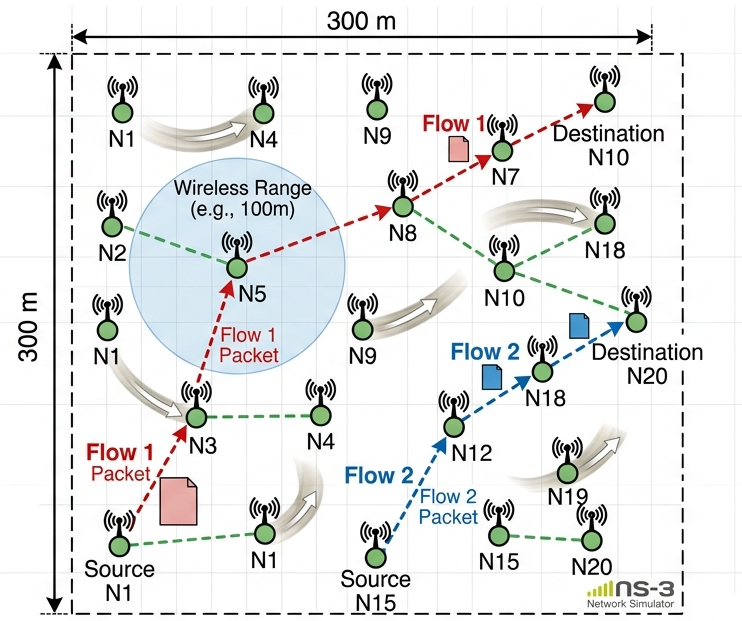
\includegraphics[width=0.70\textwidth]{figures/simulation scenerio.png}
\caption{Simulation scenario used for the comparative evaluation of AODV and OLSR in NS-3, showing the 20-node MANET environment, mobility space, and application flows.}
\label{fig:simulation-scenario}
\end{figure}

The simulation duration was 70 seconds. Application traffic was configured as UDP Constant Bit Rate (CBR), with two flows established in the scenario. Each packet had a size of 512 bytes, and traffic generation began after a 10-second warm-up period to allow the network state and node mobility to stabilise before measurements became meaningful. The same scenario settings were preserved for both routing protocols so that the comparison remained fair and controlled.

The two routing protocols evaluated in the study were Ad hoc On-Demand Distance Vector (AODV) and Optimized Link State Routing (OLSR). AODV represents a reactive routing approach in which routes are established only when required, whereas OLSR represents a proactive routing approach in which route information is maintained continuously \parencite{perkins2003aodv,clausen2003olsr}. In the experiment, each protocol was enabled separately, while all other simulation parameters remained unchanged. This ensured that differences in performance could be interpreted as protocol-related rather than scenario-related.

\subsection{Repeated Simulation Runs}

To improve the reliability of the results, the experiment was not limited to a single execution. Instead, each routing protocol was tested across 1000 simulation runs. Repeated execution is important in MANET research because node mobility and wireless interactions introduce variability across runs, meaning that a single result may reflect only one random instance rather than the broader behaviour of the protocol \parencite{campanile2020,kour2025,selim2025}.

By repeating the experiment many times under the same configured settings, the study reduces the effect of one-off randomness and provides a stronger basis for protocol comparison. This repeated-run design allows both average behaviour and comparative trends to be observed more confidently across the selected performance metrics.

\subsection{Performance Evaluation Metrics}

The performance of AODV and OLSR was evaluated using five standard metrics: packet delivery ratio, throughput, end-to-end delay, jitter, and packet loss. These metrics were selected because they provide a balanced view of routing reliability, data delivery efficiency, and temporal consistency in MANET communication \parencite{carneiro2009flowmonitor,mohapatra2012,sarao2022,selim2025}.

Packet Delivery Ratio (PDR) measures the proportion of transmitted packets that are successfully received at the destination. It is widely used as an indicator of routing reliability in MANET performance evaluation \parencite{mohapatra2012,radha2018,sarao2022}. It is calculated as:

\begin{equation}
PDR = \frac{\text{Total packets received}}{\text{Total packets sent}} \times 100
\end{equation}

Throughput measures the effective rate of successful data delivery across the network and reflects the useful data-carrying performance of the protocol \parencite{carneiro2009flowmonitor,mohapatra2012,selim2025}. It is calculated as:

\begin{equation}
Throughput = \frac{\text{Total received bytes} \times 8}{\text{Simulation time}}
\end{equation}

End-to-end delay represents the average time taken for packets to travel from source to destination. It captures the combined effect of route discovery, transmission, queuing, and forwarding delay \parencite{mohapatra2012,radha2018,sarao2022}. It is calculated as:

\begin{equation}
Delay = \frac{\sum(\text{Packet receive time} - \text{Packet send time})}{\text{Total packets received}}
\end{equation}

Jitter measures the variation in packet delay between successive packets and is useful for assessing the temporal stability of delivery \parencite{carneiro2009flowmonitor,sarao2022,selim2025}. It is calculated as:

\begin{equation}
Jitter = \frac{\sum |\text{Delay}_{i} - \text{Delay}_{i-1}|}{N-1}
\end{equation}

Packet loss represents the number of packets that fail to reach the destination and provides additional evidence of delivery inefficiency or route instability \parencite{mohapatra2012,radha2018,selim2025}. It is calculated as:

\begin{equation}
Packet\ Loss = \text{Total packets sent} - \text{Total packets received}
\end{equation}

These metrics were extracted through FlowMonitor and then processed for comparison across protocols and across repeated runs \parencite{carneiro2009flowmonitor,riley2010ns3,ns3flowmonitordocs}.

\subsection{Data Collection and Analysis Workflow}

After each simulation run, FlowMonitor was used to generate structured output containing per-flow statistics. These outputs were then processed using Python scripts to extract and organise the required performance values for both protocols. The analysis pipeline transformed raw simulation data into a comparative dataset containing throughput, packet delivery ratio, delay, jitter, and loss values for each run.

Once the metric values were extracted, graphical visualisations were produced to support interpretation of protocol behaviour across repeated runs. These visualisations were used to show differences in overall trend, average performance, and consistency between AODV and OLSR. This process made it possible to move from raw flow-level data to a more interpretable comparative analysis while preserving traceability back to the original simulation outputs.

\subsection{AI-Assisted Interpretation}

AI-assisted analysis was incorporated only after the simulation and metric extraction stages had been completed. Its role was limited to supporting the interpretation of results by helping to identify recurring patterns, organise comparative observations, and improve the clarity of written discussion. The AI component did not participate in the generation of simulation data, routing decisions, or metric computation.

This distinction is important for methodological transparency. The primary evidence in the study remains the measured outputs generated by NS-3 and FlowMonitor. AI was used only as a secondary interpretive layer to assist with analysis of those results. In this way, the study demonstrates how AI can be integrated into simulation-based networking research without compromising the validity of the original measurements \parencite{bhatia2022,duong2024,schuler2021}.

\subsection{Section Summary}

This section has presented the methodology used for the comparative evaluation of AODV and OLSR in NS-3. It explained the quantitative and simulation-based design of the study, the experimental environment, the scenario configuration, the repeated-run approach, the selected performance metrics, the data collection and analysis workflow, and the role of AI-assisted interpretation. Together, these elements establish the methodological basis for the results and discussion presented in the following sections.

\section{Simulation Implementation}

This section describes how the comparative experiment was implemented in NS-3. While the previous section defined the methodological design of the study, the present section explains how that design was translated into the actual simulation workflow, including node creation, mobility setup, traffic generation, routing protocol integration, FlowMonitor instrumentation, and post-simulation processing. The purpose of the section is to show the practical implementation of the experiment before presenting the measured results.

\subsection{NS-3 Simulation Development}

The experiment was implemented as an NS-3 simulation script designed to compare AODV and OLSR under the same MANET conditions. The script created the simulation nodes, configured the wireless environment, assigned mobility behaviour, installed the Internet stack, enabled the selected routing protocol, and generated application traffic. The implementation was structured so that the same script logic could be used for both protocols, with the routing mechanism changed between runs while the rest of the scenario remained constant. This ensured consistency across the comparative experiment.

The implementation followed a modular workflow in which scenario parameters such as node count, simulation area, mobility configuration, packet size, and simulation duration were defined explicitly. This made the script easier to repeat, modify, and validate. It also supported the repeated-run design adopted in the study by allowing the same simulation structure to be executed many times under controlled settings.

\subsection{Node Creation and Wireless Configuration}

The NS-3 script instantiated 20 mobile nodes to form the MANET environment. These nodes were configured to communicate over a wireless channel within a \(300 \times 300\) metre simulation area. The wireless setup was designed to provide a shared communication medium in which route establishment, forwarding, and route breakage could occur naturally as nodes moved within the defined space.

Each node was equipped with the protocol stack necessary for MANET communication, including network-layer support for the routing protocol under test. The wireless configuration remained unchanged between the AODV and OLSR experiments. This was important because the purpose of the study was to compare routing behaviour rather than differences introduced by alternative link-layer or physical-layer settings.

\subsection{Mobility and Traffic Configuration}

Node mobility was implemented using the Random Waypoint model. The configured speed range was 1--3 m/s, with a pause time of 2 seconds. This mobility pattern was selected to create continuous but moderate topology change, thereby exercising route discovery, route maintenance, and packet forwarding throughout the simulation period.

Application traffic was configured as UDP Constant Bit Rate (CBR). Two flows were defined in the scenario in order to generate repeatable traffic demand across the MANET. Each packet had a size of 512 bytes, and application traffic began at 10 seconds rather than at the start of the simulation. This 10-second warm-up period was included to allow node placement, mobility progression, and preliminary route formation to stabilise before measurements became significant. The total simulation time was 70 seconds.

\subsection{Routing Protocol Integration}

The comparative implementation focused on two routing protocols: AODV and OLSR. In the NS-3 script, these were enabled separately using the appropriate routing helpers, while all other parameters were preserved. This means that the network topology, node mobility, traffic flows, packet settings, and simulation duration were identical in both cases. Only the routing protocol differed between runs.

This implementation choice was central to the fairness of the experiment. Because AODV is reactive and OLSR is proactive, the comparison aimed to observe how these routing strategies behaved under the same operating conditions rather than under separate or customised scenarios. The resulting outputs therefore reflect protocol-specific behaviour within a common implementation framework.

\subsection{FlowMonitor Instrumentation}

FlowMonitor was integrated into the simulation to capture flow-level performance information after each run. Its purpose was to record measurable statistics such as transmitted packets, received packets, cumulative delay, jitter-related information, and packet loss. This made it possible to collect comparable performance data for both protocols using a consistent monitoring mechanism.

At the end of each simulation run, FlowMonitor generated structured output that could be exported and analysed further. This instrumentation step formed the bridge between simulation execution and metric computation. Rather than relying only on console output or manual observation, the experiment used FlowMonitor to provide a reproducible measurement basis for packet delivery ratio, throughput, delay, jitter, and loss.

\subsection{Repeated Execution Workflow}

The simulation was executed repeatedly for both routing protocols in order to reduce dependence on a single random outcome. Each protocol was run 1000 times under the same configured scenario. This repeated execution process was important because mobility-driven MANET experiments can produce variable outcomes across runs due to differences in movement patterns and resulting route dynamics.

To support this repeated-run workflow, outputs were generated and organised in a way that allowed later aggregation and comparison. Each run contributed to the overall dataset for the protocol being tested, making it possible to evaluate average behaviour and broader performance trends rather than relying on isolated results.

\subsection{Output Parsing and Metric Computation}

After simulation execution, the FlowMonitor outputs were processed using Python. The parsing stage extracted the relevant flow-level values required for the performance evaluation, including packet counts, received bytes, delay totals, and jitter totals. These extracted values were then used to compute the final comparison metrics for each run.

From the processed outputs, packet delivery ratio, throughput, average delay, jitter, and packet loss were calculated and stored in a structured format. This made it possible to summarise results by protocol and compare their behaviour across the full set of repeated runs. The use of Python also supported automation and reduced the likelihood of manual calculation errors in the post-simulation stage.

\subsection{Graph Generation and Comparative Preparation}

Once the performance metrics had been computed, the processed dataset was used to generate graphs for comparative analysis. These visualisations were designed to show how AODV and OLSR differed across the selected metrics and how stable their behaviour appeared over repeated runs. Graph generation therefore served two purposes: it supported clearer interpretation of the results and provided an accessible way to present protocol-level performance differences in the results section.

In addition to individual metric plots, the processed outputs also supported summary comparison of both protocols. This prepared the dataset for the final stages of the study, where measured values, visual trends, and comparative observations were brought together for interpretation.

\subsection{AI-Assisted Interpretation Workflow}

After the simulation data had been parsed and the performance metrics had been computed, AI-assisted analysis was applied as a secondary interpretive step. The extracted results were supplied to the AI component in structured form so that it could help identify comparative trends, organise observations, and support the articulation of findings. This stage was analytical rather than generative in the experimental sense.

Importantly, the AI component did not participate in node mobility, traffic generation, route computation, or metric calculation. Its role began only after the measured outputs were already available. This preserved the distinction between primary simulation evidence and secondary interpretive support, ensuring that the comparative evaluation remained grounded in the NS-3 and FlowMonitor outputs.

\subsection{Section Summary}

This section has described how the comparative study was implemented in practice within NS-3. It has outlined the creation of the 20-node MANET scenario, the wireless and mobility setup, the UDP CBR traffic configuration, the separate integration of AODV and OLSR, the use of FlowMonitor for data collection, the repeated-run execution process, and the Python-based parsing and graph generation workflow. It has also clarified the limited role of AI-assisted interpretation in the overall process. Together, these implementation details provide the practical basis for the results presented in the next section.

\section{Results}

This section presents the measured results of the comparative evaluation of AODV and OLSR in NS-3. The results are based on FlowMonitor-derived metrics aggregated across 1000 simulation runs per protocol, using the scenario defined earlier in the study. The analysis focuses on throughput, packet delivery ratio, end-to-end delay, jitter, and packet loss, with application-flow consistency included to qualify the fairness of interpretation. The aggregated outputs show that AODV achieved higher throughput, whereas OLSR achieved better packet delivery ratio, lower packet loss, lower average delay, and lower average jitter. The results also show that AODV maintained the configured application-flow count more consistently than OLSR.

\subsection{Overview of Aggregate Results}

The final summary metrics indicate a mixed outcome rather than a single absolute winner. Table~\ref{tab:aggregate-results} summarises the aggregate performance values extracted from the final CSV outputs. AODV achieved higher average throughput, whereas OLSR achieved stronger packet delivery ratio, lower packet loss, lower average delay, and lower average jitter. At the same time, AODV preserved the configured traffic pattern more consistently, with an average application-flow count of 2.000 compared with 1.264 for OLSR. These values were generated from the summary export stage of the analysis workflow and reflect the aggregate results across 1000 runs per protocol.

These results show that the two protocols exhibited different strengths under the configured scenario. AODV produced higher data-transfer rate and stronger flow consistency, whereas OLSR produced better delivery efficiency and lower temporal instability across the active flows observed. This means the results should be interpreted comparatively rather than reduced to a single overall protocol winner.

\begin{table}[htbp]
\centering
\caption{Aggregate performance summary for AODV and OLSR across 1000 simulation runs per protocol}
\label{tab:aggregate-results}
\begin{tabular}{lcc}
\toprule
\textbf{Metric} & \textbf{AODV} & \textbf{OLSR} \\
\midrule
Runs & 1000 & 1000 \\
Average application-flow count & 2.000 & 1.264 \\
Average throughput (Mbps) & 0.4188 & 0.3282 \\
Packet delivery ratio (\%) & 23.16 & 52.26 \\
Packet loss (\%) & 76.84 & 34.54 \\
Average delay (ms) & 86.72 & 57.87 \\
Average jitter (ms) & 2.89 & 1.34 \\
\bottomrule
\end{tabular}
\end{table}

\subsection{Throughput Results}

Figure~\ref{fig:throughput-results} presents the average throughput achieved by AODV and OLSR. The results show that AODV outperformed OLSR in average throughput under the configured MANET scenario. Across the 1000-run aggregate, AODV achieved approximately 0.4188 Mbps, while OLSR achieved approximately 0.3282 Mbps. This indicates that AODV maintained a higher rate of successful data delivery in the active flows observed during the experiment.

Although AODV achieved stronger throughput, this result must be considered alongside the other delivery metrics reported later in this section. Higher throughput in this case does not automatically imply better overall routing quality, since packet delivery ratio and packet loss show a different pattern of protocol performance. The throughput result therefore highlights one aspect of protocol behaviour rather than a complete performance judgement.

\begin{figure}[htbp]
\centering
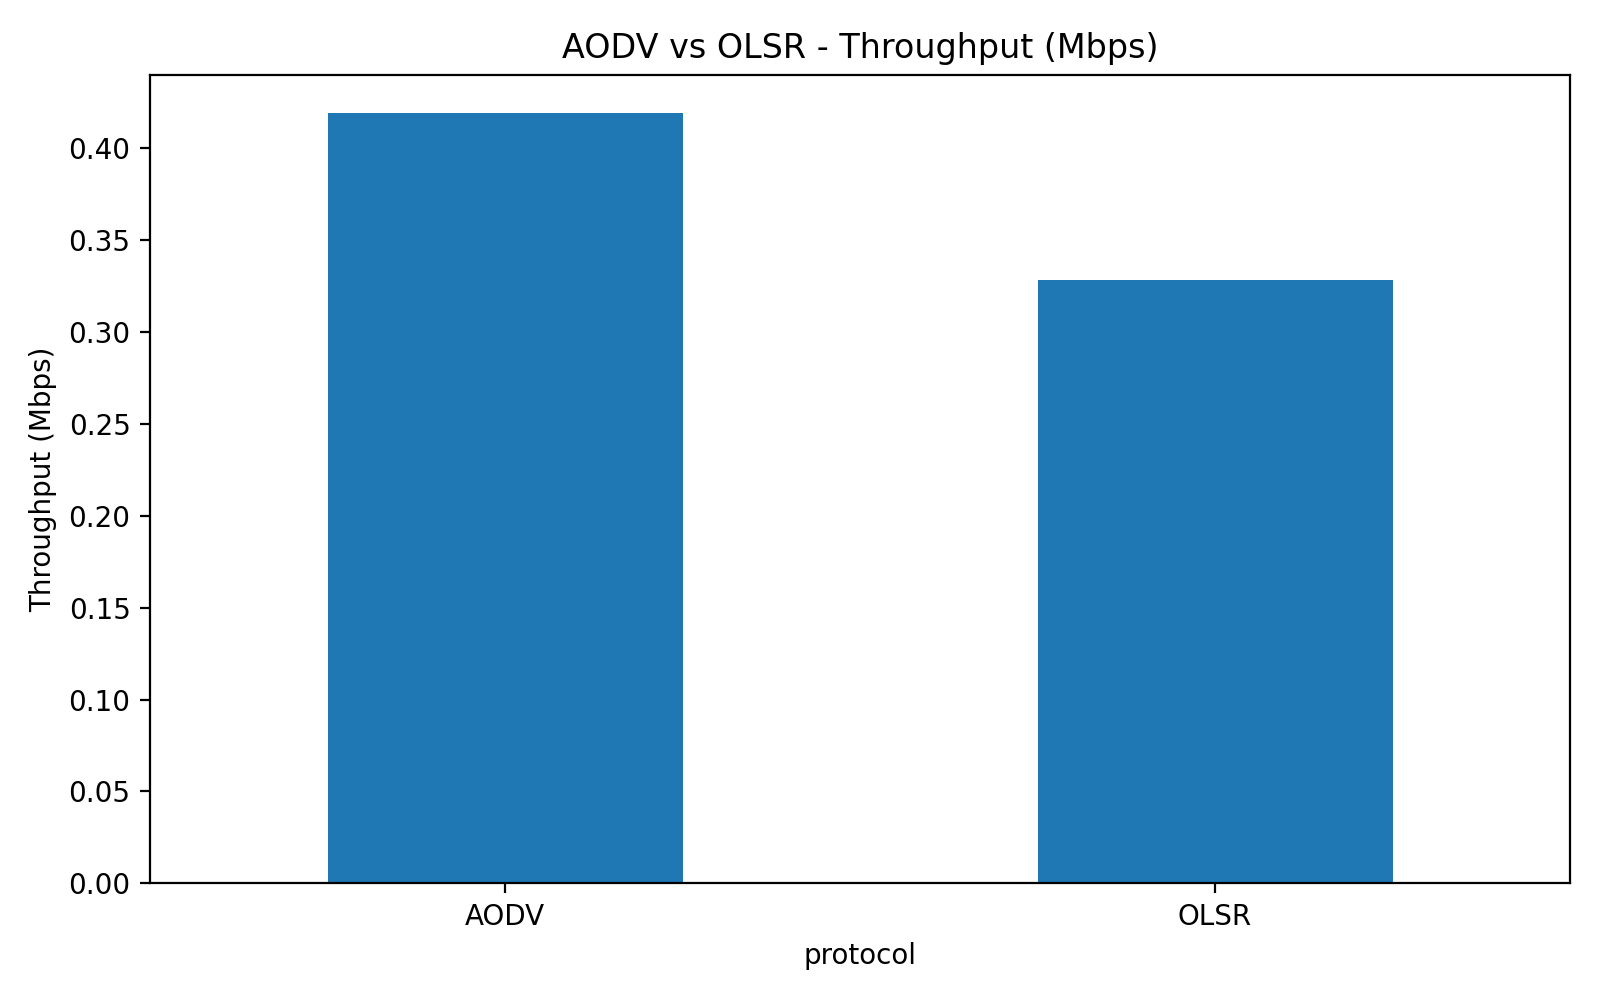
\includegraphics[width=0.70\textwidth]{figures/throughput_mbps.png}
\caption{Average throughput comparison between AODV and OLSR.}
\label{fig:throughput-results}
\end{figure}

\subsection{Packet Delivery Ratio Results}

Figure~\ref{fig:pdr-results} presents the packet delivery ratio achieved by the two routing protocols. In contrast to the throughput result, OLSR performed substantially better than AODV in terms of delivery success. OLSR achieved an average packet delivery ratio of 52.26\%, while AODV achieved 23.16\%. This represents the largest difference observed among the reported metrics and indicates that OLSR was more effective at ensuring successful packet delivery across the active flows present during the experiment.

\begin{figure}[H]
\centering
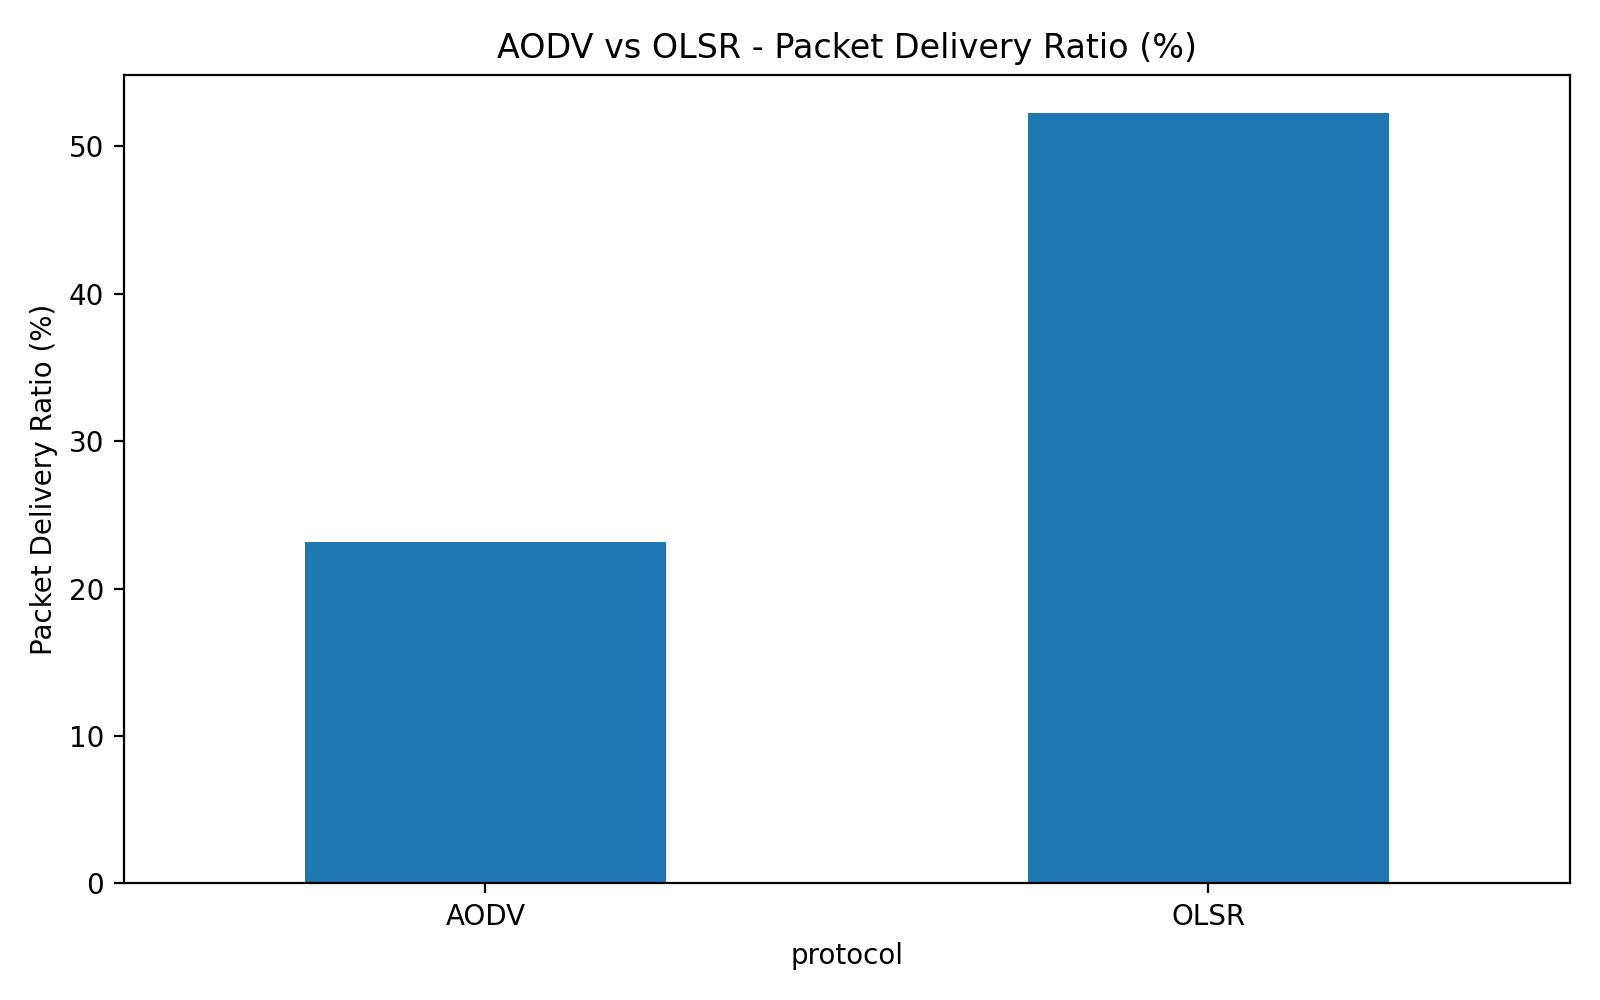
\includegraphics[width=0.70\textwidth]{figures/pdr_percent.png}
\caption{Packet delivery ratio comparison between AODV and OLSR.}
\label{fig:pdr-results}
\end{figure}

The packet delivery result is important because it directly reflects routing reliability. While AODV carried more data in terms of throughput, OLSR delivered a substantially higher proportion of the transmitted packets. This suggests that under the configured mobility and traffic conditions, OLSR maintained more dependable active delivery paths than AODV.

\subsection{Delay Results}

Figure~\ref{fig:delay-results} shows the average end-to-end delay recorded for AODV and OLSR. The results indicate that OLSR achieved lower delay than AODV across the repeated runs. The average delay for OLSR was 57.87 ms, whereas AODV recorded 86.72 ms. This means that packets delivered under OLSR generally reached their destination faster than those delivered under AODV.

\begin{figure}[htbp]
\centering
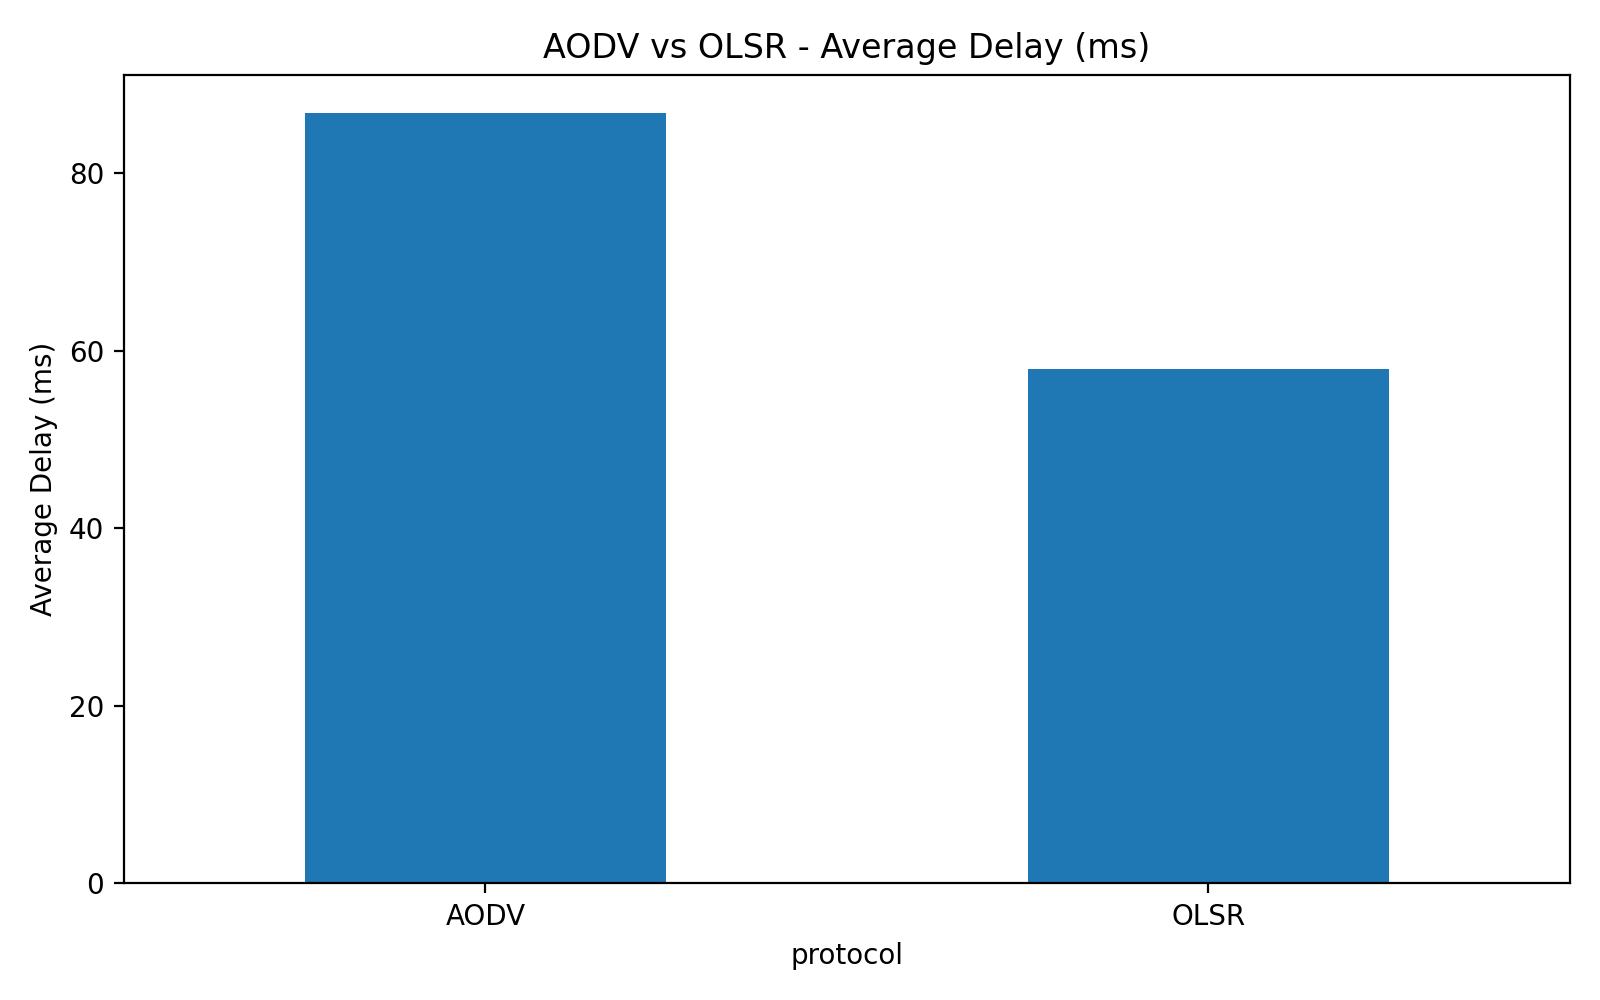
\includegraphics[width=0.70\textwidth]{figures/avg_delay_ms.png}
\caption{Average end-to-end delay comparison between AODV and OLSR.}
\label{fig:delay-results}
\end{figure}

This result is consistent with the idea that proactive route availability can reduce waiting time before forwarding begins. In descriptive terms, the delay outcome shows that OLSR supported more time-efficient delivery in the flows that remained active, while AODV experienced greater timing overhead under the same scenario conditions.

\subsection{Jitter Results}

Figure~\ref{fig:jitter-results} presents the average jitter values for the two protocols. OLSR again performed better, with an average jitter of 1.34 ms compared with 2.89 ms for AODV. Since jitter reflects variation in packet delay, this result indicates that OLSR provided more temporally stable packet delivery than AODV across the repeated simulation runs.

\begin{figure}[H]
\centering
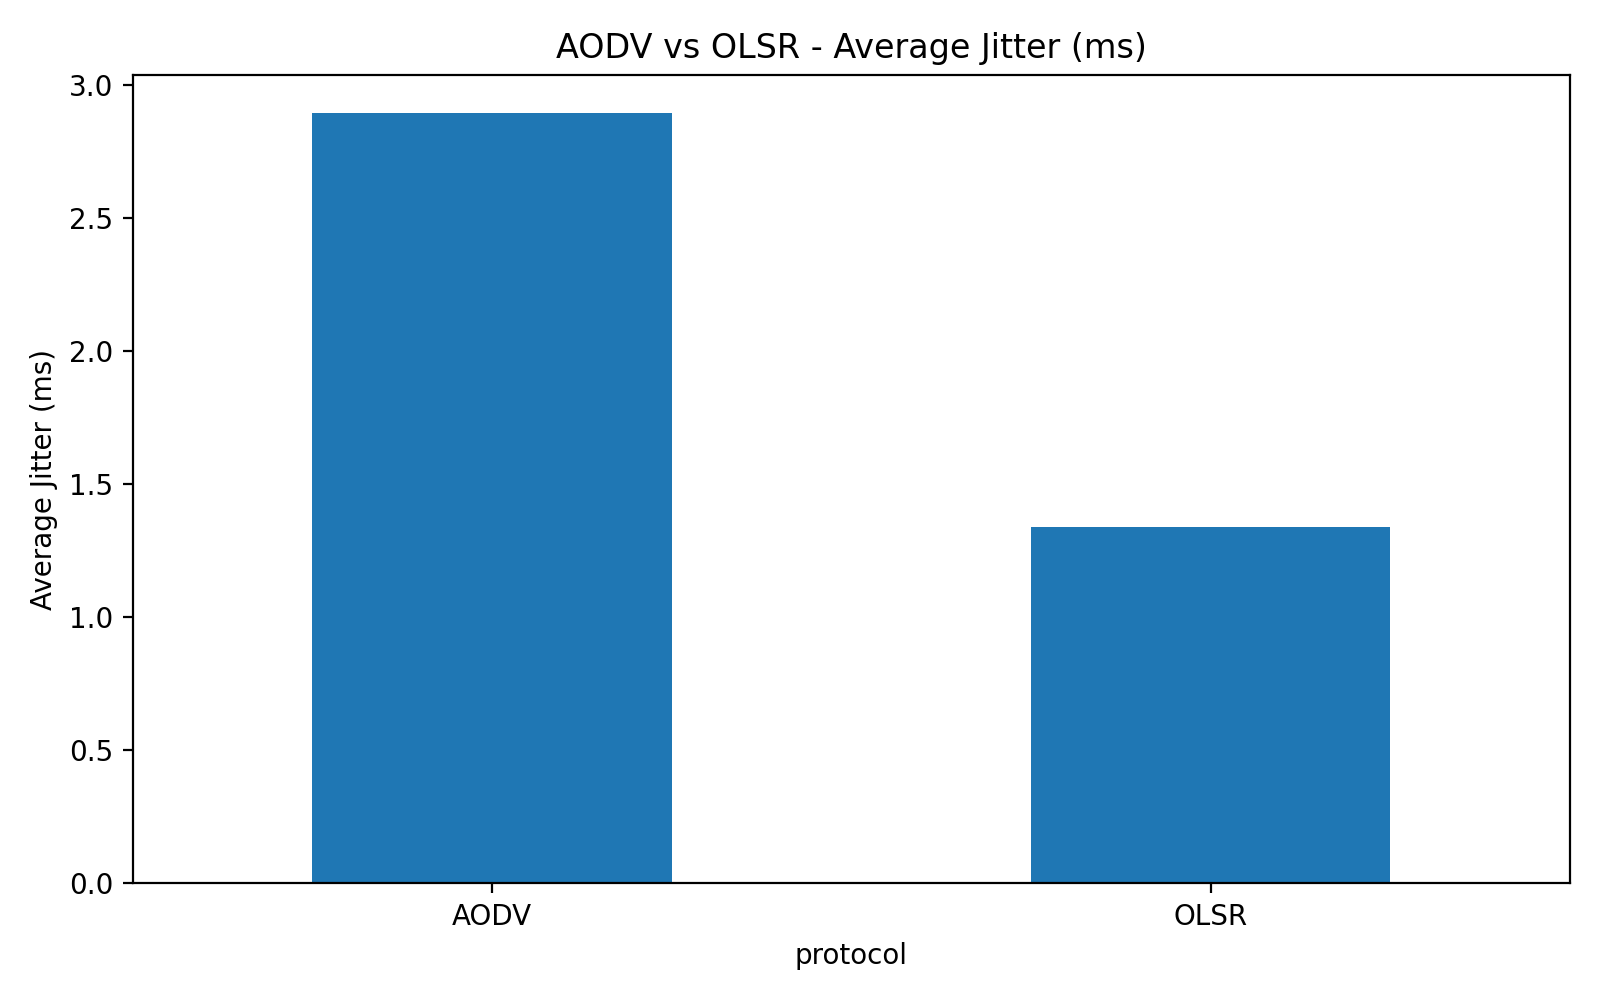
\includegraphics[width=0.70\textwidth]{figures/avg_jitter_ms.png}
\caption{Average jitter comparison between AODV and OLSR.}
\label{fig:jitter-results}
\end{figure}

Lower jitter is important because it suggests more consistent packet arrival over time. In this experiment, OLSR not only achieved lower delay but also lower delay variation, which strengthens the evidence that it produced more stable delivery behaviour under the configured MANET conditions.

\subsection{Packet Loss Results}

Figure~\ref{fig:loss-results} shows the average packet loss percentages observed for the two protocols. OLSR recorded substantially lower loss than AODV, with an average value of 34.54\% compared with 76.84\% for AODV. This result corresponds closely with the packet delivery ratio findings and further confirms that OLSR was more effective in retaining packet delivery under the selected simulation scenario.

\begin{figure}[H]
\centering
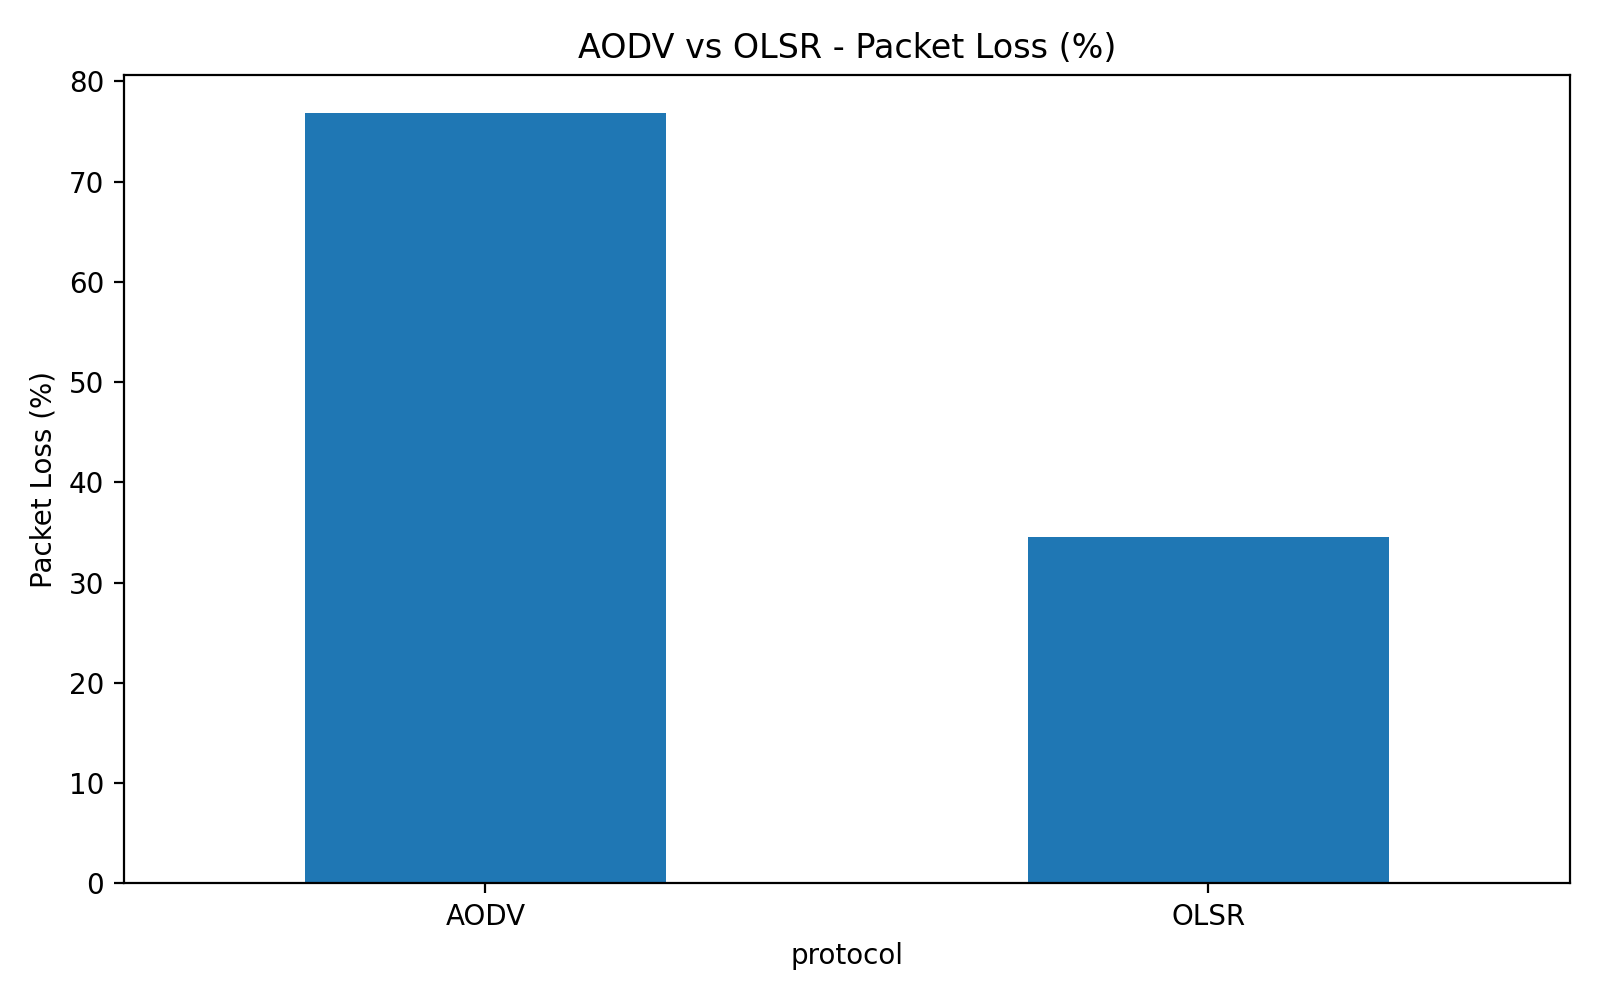
\includegraphics[width=0.70\textwidth]{figures/loss_percent.png}
\caption{Packet loss comparison between AODV and OLSR.}
\label{fig:loss-results}
\end{figure}

The loss result reinforces the view that the higher throughput achieved by AODV should not be interpreted in isolation. Although AODV transferred data at a higher average rate, it also lost a far greater proportion of packets than OLSR. This means OLSR provided stronger packet retention and more reliable forwarding within the active flows captured in the experiment.

\subsection{Application Flow Consistency}

Figure~\ref{fig:flowcount-results} presents the average application-flow count observed for each protocol. This metric is important because it affects how the other performance outcomes should be interpreted. AODV maintained the configured number of application flows consistently, producing an average value of 2.000, while OLSR produced an average value of 1.264. This indicates that OLSR’s stronger delivery performance was achieved under a lower average count of active application flows.

\begin{figure}[H]
\centering
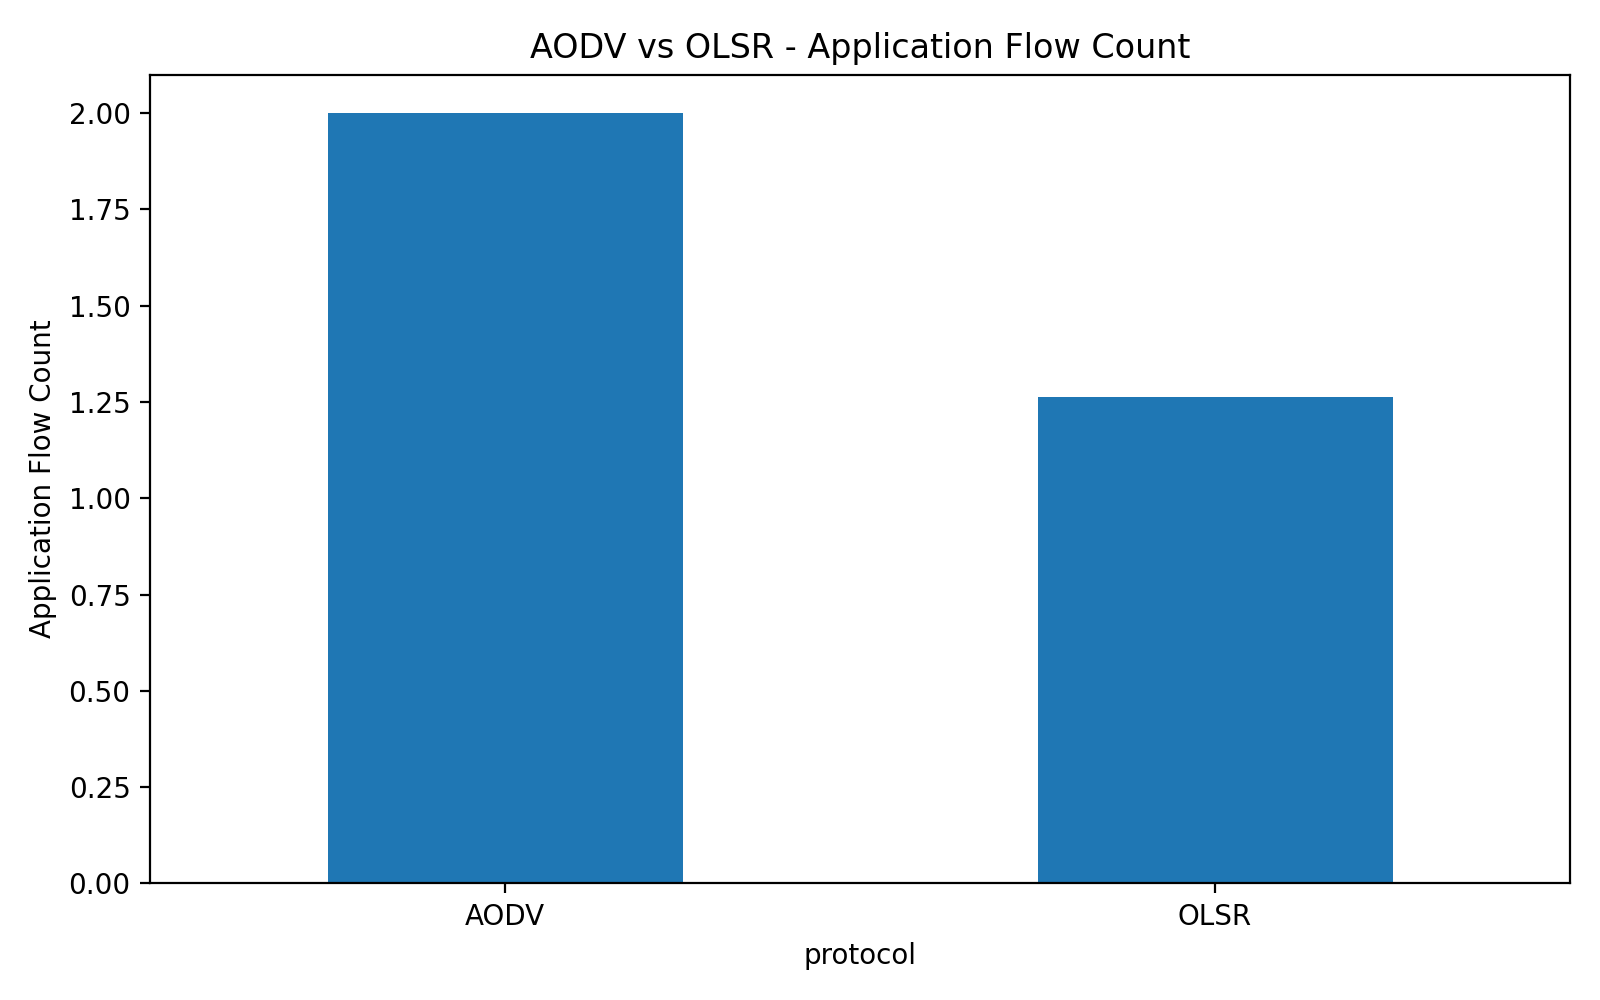
\includegraphics[width=0.70\textwidth]{figures/application_flow_count.png}
\caption{Average application-flow count comparison between AODV and OLSR.}
\label{fig:flowcount-results}
\end{figure}

This observation introduces an important fairness consideration. On one hand, OLSR clearly outperformed AODV in packet delivery ratio, packet loss, delay, and jitter. On the other hand, AODV preserved the configured traffic pattern more consistently across runs. The results should therefore be interpreted with care: OLSR showed better per-flow delivery quality, while AODV showed stronger flow persistence under the tested conditions.

\subsection{Additional Distribution-Based Results}

Beyond the main comparison graphs presented in this section, additional distribution-based visualisations were generated to examine spread, central tendency, and variability across repeated runs. These include boxplots, histograms, error-bar plots, and line plots for the evaluated metrics. To preserve clarity in the main body of the report, these supporting figures are provided in the Appendix. Their purpose is to complement the aggregate results shown here rather than replace them.

\subsection{Overall Comparative Summary}

To complement the individual metric graphs, Figure~\ref{fig:results-infographic} provides a consolidated visual summary of the comparative performance of AODV and OLSR across the evaluated metrics. The infographic highlights that AODV achieved stronger throughput and application-flow consistency, whereas OLSR achieved better packet delivery ratio, lower packet loss, lower delay, and lower jitter. This figure is intended as a high-level synthesis of the results already presented in detail, rather than as a replacement for the metric-specific analysis.

\begin{figure}[htbp]
\centering
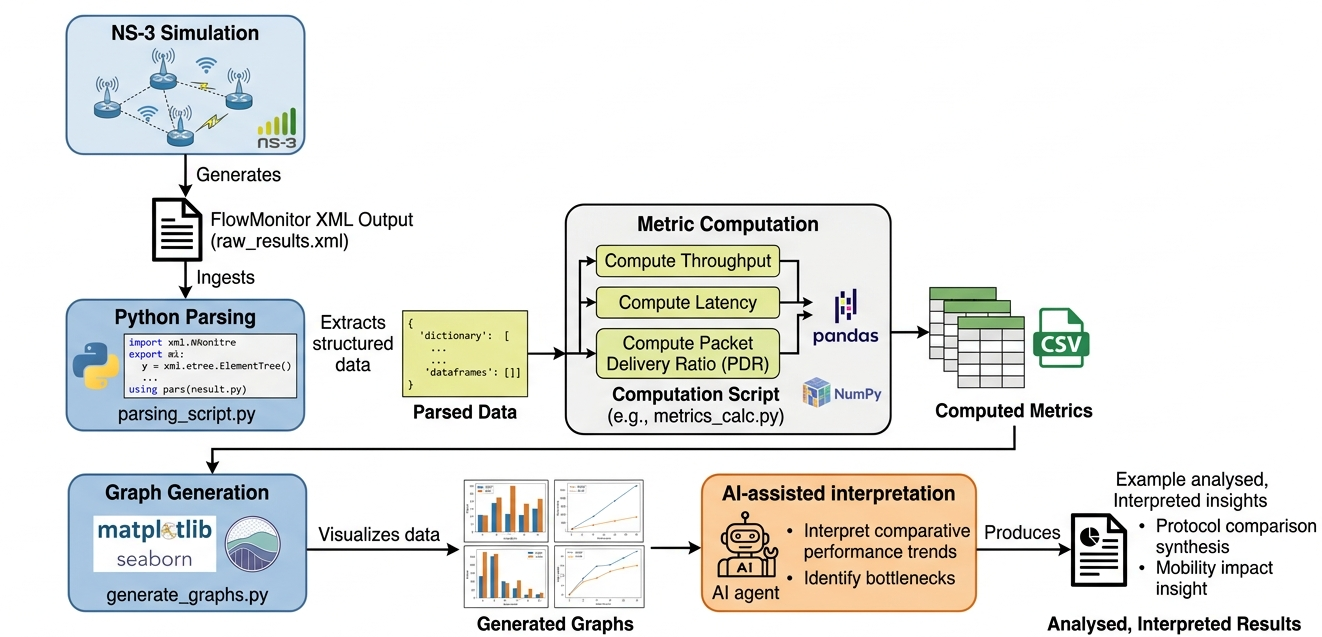
\includegraphics[width=1\textwidth]{figures/Results_infographic.png}
\caption{Overall comparative summary of AODV and OLSR performance across the evaluated metrics.}
\label{fig:results-infographic}
\end{figure}

\subsection{Section Summary}

This section has presented the measured results of the comparative evaluation of AODV and OLSR across 1000 simulation runs per protocol. The results show that AODV achieved higher throughput and stronger application-flow consistency, whereas OLSR achieved higher packet delivery ratio, lower packet loss, lower delay, and lower jitter. The findings therefore indicate that protocol performance depended on the criterion being considered, and that the lower average active-flow count observed for OLSR should be taken into account when interpreting the comparison. The overall comparative infographic further reinforces this result by summarising the differing strengths of both protocols in a single visual form. These results provide the basis for the analytical discussion in the next section.

\section{Discussion}

This section interprets the results of the comparative evaluation of AODV and OLSR in relation to the routing behaviour of both protocols and the broader MANET literature. Rather than identifying a single absolute winner, the discussion considers how the observed differences reflect the trade-off between reactive and proactive routing under the configured NS-3 scenario. Particular attention is given to the fact that AODV achieved higher throughput and stronger application-flow consistency, whereas OLSR achieved better packet delivery ratio, lower packet loss, lower delay, and lower jitter.

\subsection{Interpretation of AODV Performance}

AODV achieved the higher average throughput in the experiment, which indicates that it maintained a stronger rate of successful data transfer across the active flows observed. This result is consistent with the reactive nature of AODV, where routes are created only when needed rather than maintained continuously. Under some conditions, this can reduce unnecessary routing overhead and allow more of the available channel capacity to be used for application traffic \parencite{perkins2003aodv,belding2003,midha2013}.

However, AODV also recorded lower packet delivery ratio, higher packet loss, higher delay, and higher jitter than OLSR. This suggests that although AODV could support stronger data-transfer rate when flows remained active, it was less effective at preserving reliable and stable packet forwarding under the configured mobility conditions. A likely explanation is that the on-demand route discovery process introduced route acquisition and recovery penalties as the topology changed, thereby increasing timing instability and reducing overall delivery success \parencite{chakeres2004,mohapatra2012,bappalige2020}.

The application-flow result also favoured AODV, with an average flow count of 2.000 compared with 1.264 for OLSR. This indicates that AODV preserved the configured traffic structure more consistently across the repeated runs. As a result, AODV’s performance cannot be described simply as poor; rather, it showed strength in throughput and flow persistence, but weakness in delivery reliability and temporal stability under the tested scenario.

\subsection{Interpretation of OLSR Performance}

OLSR outperformed AODV in packet delivery ratio, packet loss, average delay, and average jitter. This pattern indicates that OLSR provided more reliable and more temporally stable packet delivery across the active flows observed in the experiment. Such an outcome is consistent with the proactive nature of OLSR, in which route information is maintained continuously rather than being created only after demand arises \parencite{clausen2003olsr,clausen2011nhdp,clausen2014olsrv2}.

Because routes are already available at the moment traffic must be forwarded, OLSR can reduce the waiting time associated with route discovery. This offers a plausible explanation for the lower average delay observed in the results. In addition, the lower jitter suggests that OLSR supported more stable packet arrival over time, which is important in dynamic wireless environments where route fluctuations can easily disrupt delivery consistency \parencite{spaho2013,wheeb2023,sarkar2025}.

Despite these advantages, OLSR did not outperform AODV in throughput and did not maintain the configured flow count as consistently. This is an important qualification. The stronger delivery metrics achieved by OLSR should therefore be interpreted as evidence of better per-flow delivery quality, not necessarily as evidence of stronger traffic persistence or higher aggregate transfer rate under all conditions.

\subsection{Comparative Interpretation of AODV and OLSR}

Taken together, the results show that the comparison between AODV and OLSR is best understood as a trade-off between throughput and flow persistence on one side, and delivery reliability and temporal stability on the other. AODV achieved higher throughput and preserved the configured number of application flows more consistently, while OLSR achieved better packet delivery ratio, lower loss, lower delay, and lower jitter.

This outcome reinforces an important principle in MANET research: protocol performance depends strongly on the criterion being considered. If the primary requirement is higher data-transfer rate and stronger flow continuity under the configured traffic pattern, AODV appears more favourable. If the requirement is stronger delivery reliability and lower temporal instability, OLSR appears more suitable. The results therefore do not support a simplistic claim that one protocol is universally superior. Instead, they show that protocol suitability depends on what aspect of performance is prioritised \parencite{radha2018,kurniawan2020,sarkar2025,selim2025}.

A further point of interpretation concerns fairness. The lower average application-flow count observed for OLSR means that its stronger delivery metrics were achieved under a lower active-flow average than AODV. This does not invalidate the OLSR results, but it does mean that the comparison should be interpreted carefully. OLSR demonstrated better quality within the flows that remained active, whereas AODV demonstrated stronger consistency in maintaining the intended traffic pattern.

\subsection{Relationship to Existing Literature}

The findings of this study are broadly consistent with the established view that AODV and OLSR perform differently depending on mobility conditions, flow behaviour, and evaluation criteria. Prior comparative studies have similarly reported that reactive and proactive protocols do not exhibit identical strengths across all metrics, and that conclusions vary according to the simulation scenario \parencite{spaho2013,sallam2015,sallum2018,wang2022}. In this respect, the present study aligns with the broader literature by showing that protocol assessment must remain context-sensitive.

The stronger delivery efficiency observed for OLSR in this experiment is consistent with studies that associate proactive routing with improved route availability and lower latency under conditions where continuous topology knowledge is beneficial \parencite{spaho2013,radha2018,wheeb2023}. Likewise, the stronger throughput and flow persistence observed for AODV are consistent with the idea that on-demand routing can reduce unnecessary control maintenance and preserve channel resources for traffic delivery in some situations \parencite{midha2013,bappalige2020}.

At the same time, the present study contributes an additional qualification through the application-flow consistency result. This metric shows that even when one protocol appears stronger in the conventional delivery metrics, the interpretation may still require caution if the active traffic pattern differs between protocols. In that sense, the study extends the comparison beyond simple metric ranking and highlights the importance of evaluating result fairness alongside aggregate performance.

\subsection{Contribution of AI-Assisted Interpretation}

AI-assisted analysis played a limited but useful role in this study. Its purpose was not to generate the experimental evidence, but to assist with pattern recognition, comparative organisation, and the clear articulation of the results after the simulation data had already been measured. This helped support a more structured interpretation of the relationship between throughput, packet delivery ratio, packet loss, delay, jitter, and application-flow consistency.

The value of this approach lies in its ability to strengthen analytical clarity without replacing the underlying quantitative basis of the work. In this study, AI-assisted interpretation was particularly useful in identifying the need to balance protocol quality against fairness considerations in the comparison. This aligns with growing interest in combining traditional network evaluation with intelligent analytical support, while still maintaining the distinction between measured evidence and interpretive assistance \parencite{bhatia2022,duong2024,schuler2021}.

\subsection{Limitations and Future Work}

The findings of this study should be interpreted within the limits of the configured simulation scenario. The experiment used a single mobility model, a fixed terrain size, a fixed node count, a fixed packet size, and two configured UDP CBR flows. Different mobility patterns, traffic loads, node densities, or simulation durations could produce different outcomes. The conclusions are therefore valid for the present experimental setup rather than as universal rankings of AODV and OLSR performance \parencite{kour2025,sarkar2025,selim2025}.

Future work could extend the study by introducing additional routing protocols, larger node populations, different mobility models, or more demanding traffic profiles. It would also be valuable to investigate whether the application-flow disparity observed in this study persists under other parameter settings. Further work could incorporate more formal statistical testing across runs and explore more advanced forms of AI-supported post-processing while preserving the same commitment to transparency and evidence-based interpretation.

\subsection{Section Summary}

This section has interpreted the comparative results of AODV and OLSR in relation to their routing behaviour and to the wider MANET literature. The discussion showed that AODV performed better in throughput and flow persistence, whereas OLSR performed better in packet delivery ratio, loss, delay, and jitter. It also showed that the lower active-flow count observed for OLSR should be considered when assessing fairness. Overall, the findings support a criterion-dependent interpretation of protocol suitability rather than a single universal winner.
\newpage

\clearpage
\appendix

\FloatBarrier
\section{Additional Distribution-Based Figures}
\label{app:figures}

This section presents supplementary graphs generated from the repeated-run analysis. These figures complement the aggregate results discussed in the main Results section by showing variability, spread, and run-level behaviour across the 1000 simulation runs completed for each protocol. The appendix figures are grouped into boxplots, histograms, error-bar plots, and run-order line plots in order to show the distributional and temporal characteristics of the measured metrics more clearly.

\subsection{Boxplots}

The boxplots in this subsection provide a compact summary of the spread and central tendency of the measured values across repeated runs. They are useful for identifying median behaviour, interquartile range, and the presence of variability or potential outliers in the protocol results.

\begin{figure}[htbp]
\centering
\begin{subfigure}[t]{0.48\textwidth}
    \centering
    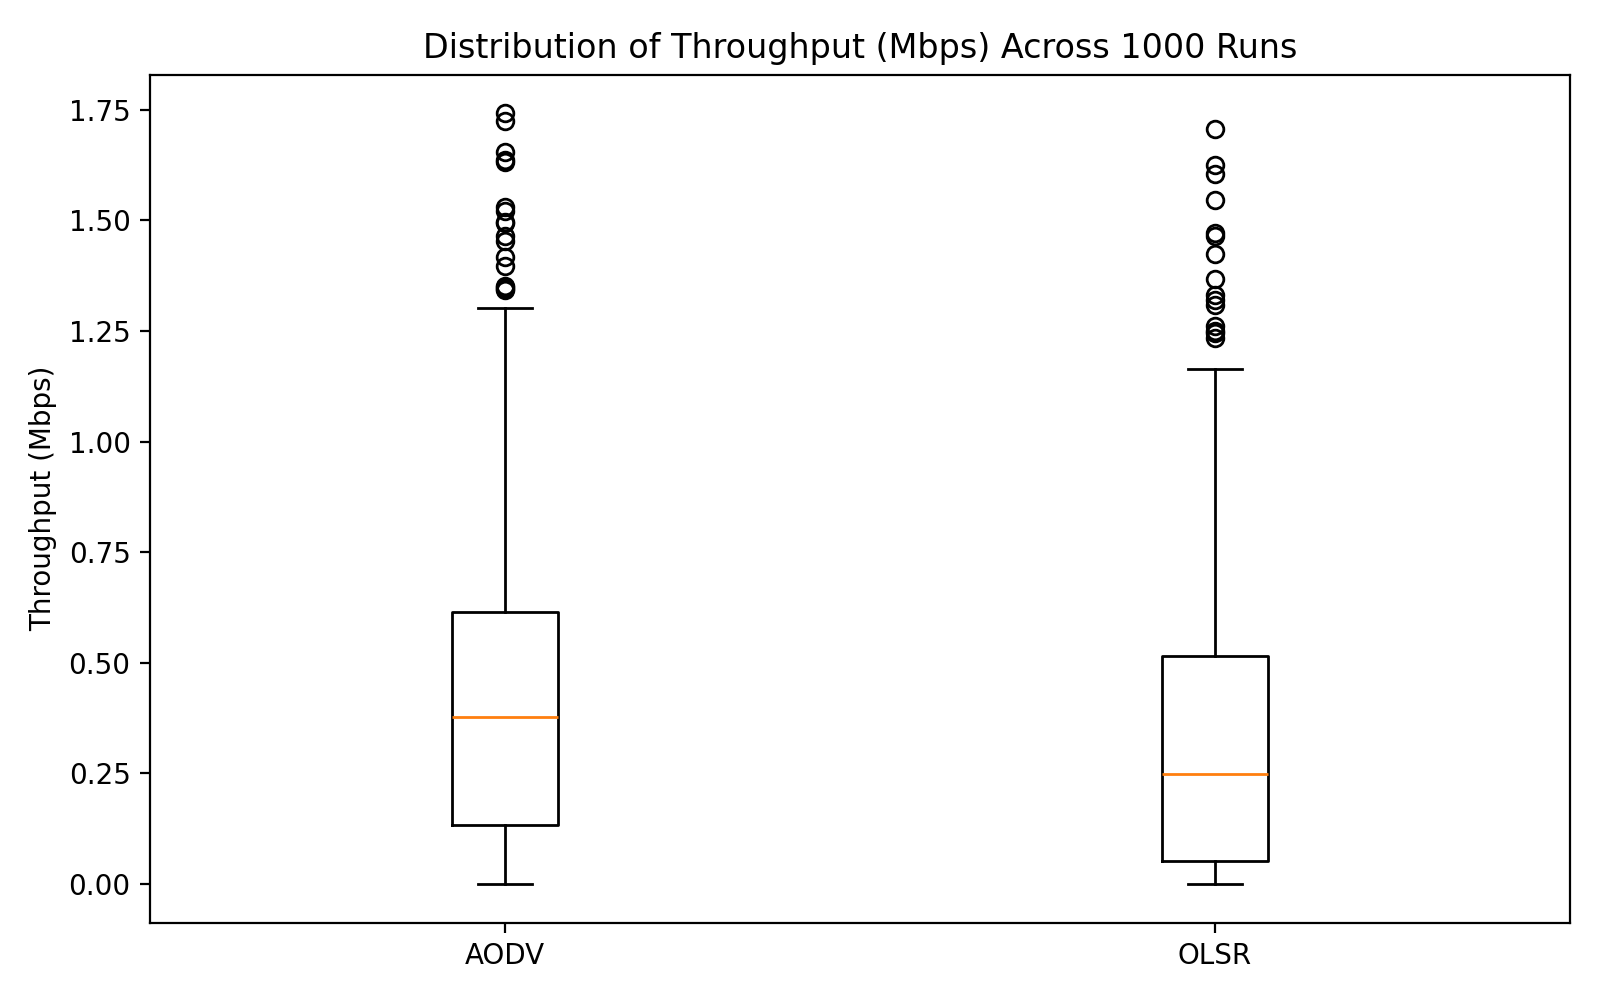
\includegraphics[width=\textwidth]{figures/boxplot_throughput_mbps.png}
    \caption{Throughput}
    \label{fig:app-box-throughput}
\end{subfigure}
\hfill
\begin{subfigure}[t]{0.48\textwidth}
    \centering
    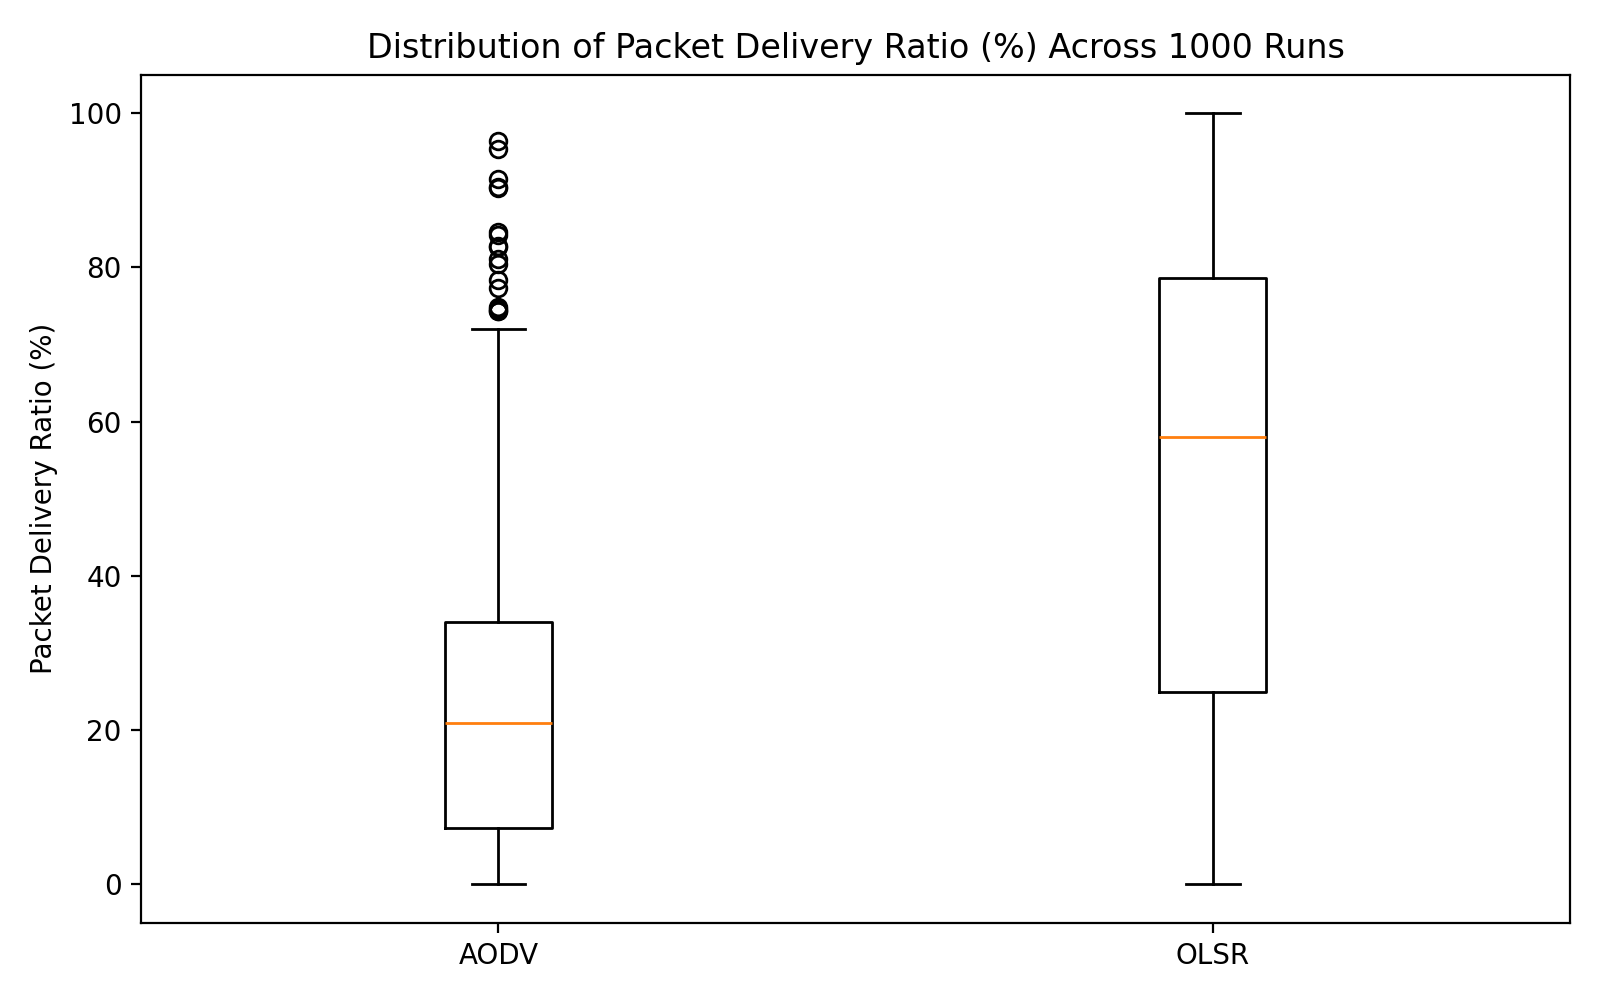
\includegraphics[width=\textwidth]{figures/boxplot_pdr_percent.png}
    \caption{Packet delivery ratio}
    \label{fig:app-box-pdr}
\end{subfigure}
\caption{Boxplot comparison of throughput and packet delivery ratio across repeated runs.}
\label{fig:app-box-1}
\end{figure}

\begin{figure}[htbp]
\centering
\begin{subfigure}[t]{0.48\textwidth}
    \centering
    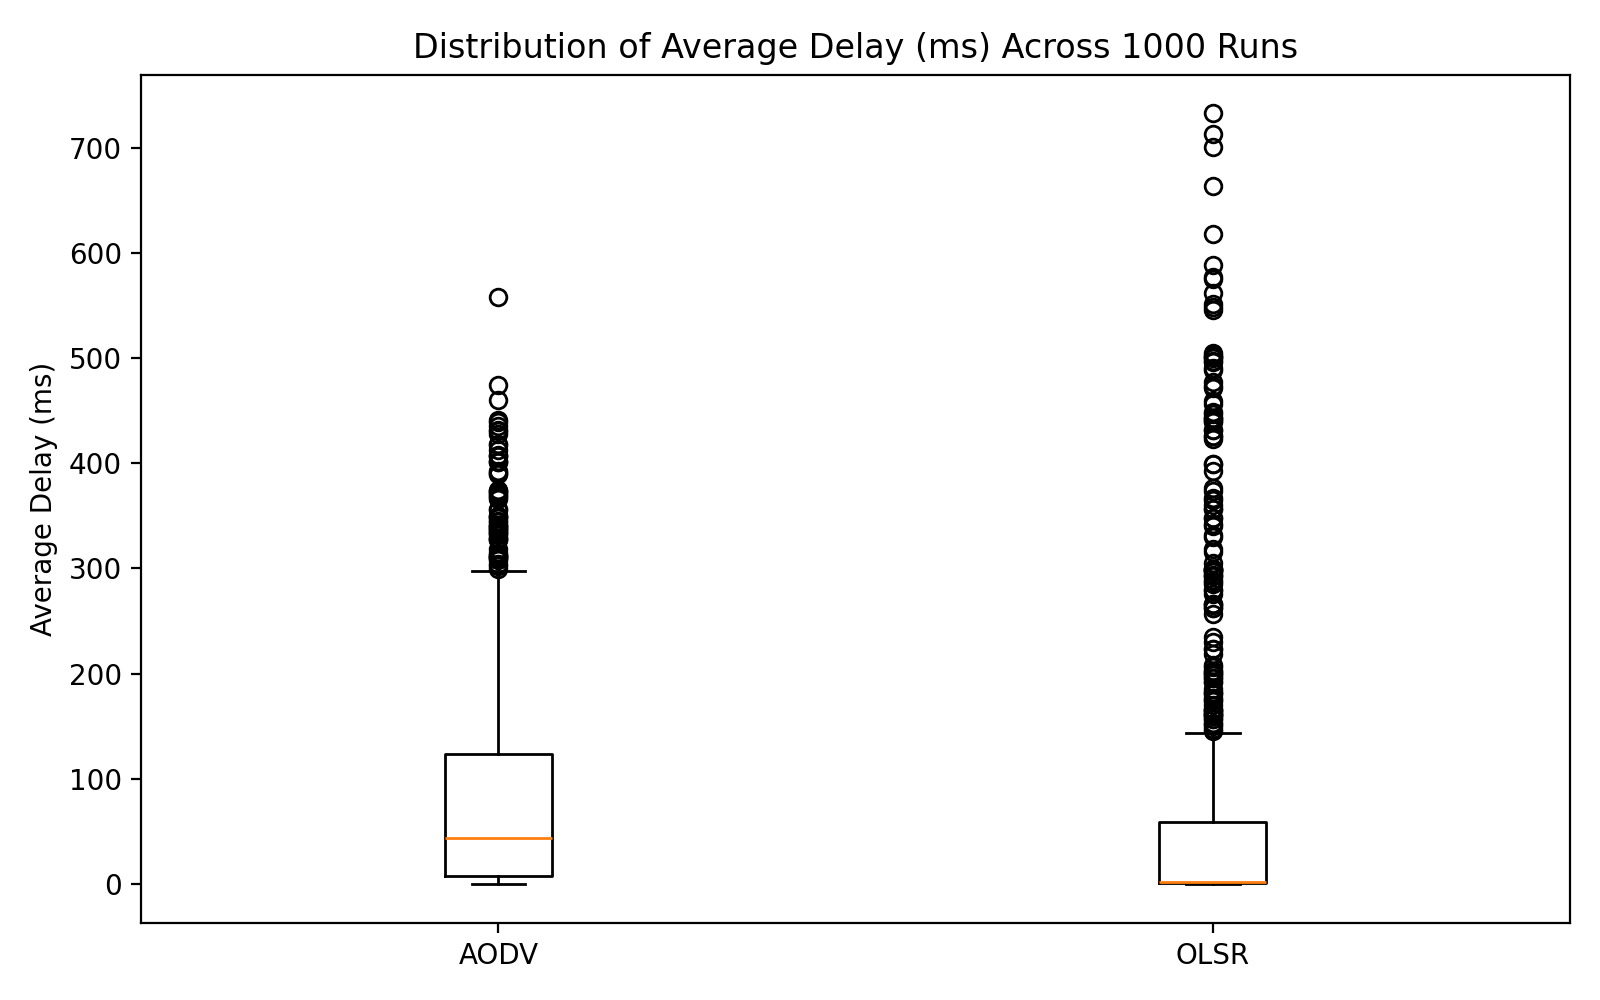
\includegraphics[width=\textwidth]{figures/boxplot_avg_delay_ms.png}
    \caption{Average delay}
    \label{fig:app-box-delay}
\end{subfigure}
\hfill
\begin{subfigure}[t]{0.48\textwidth}
    \centering
    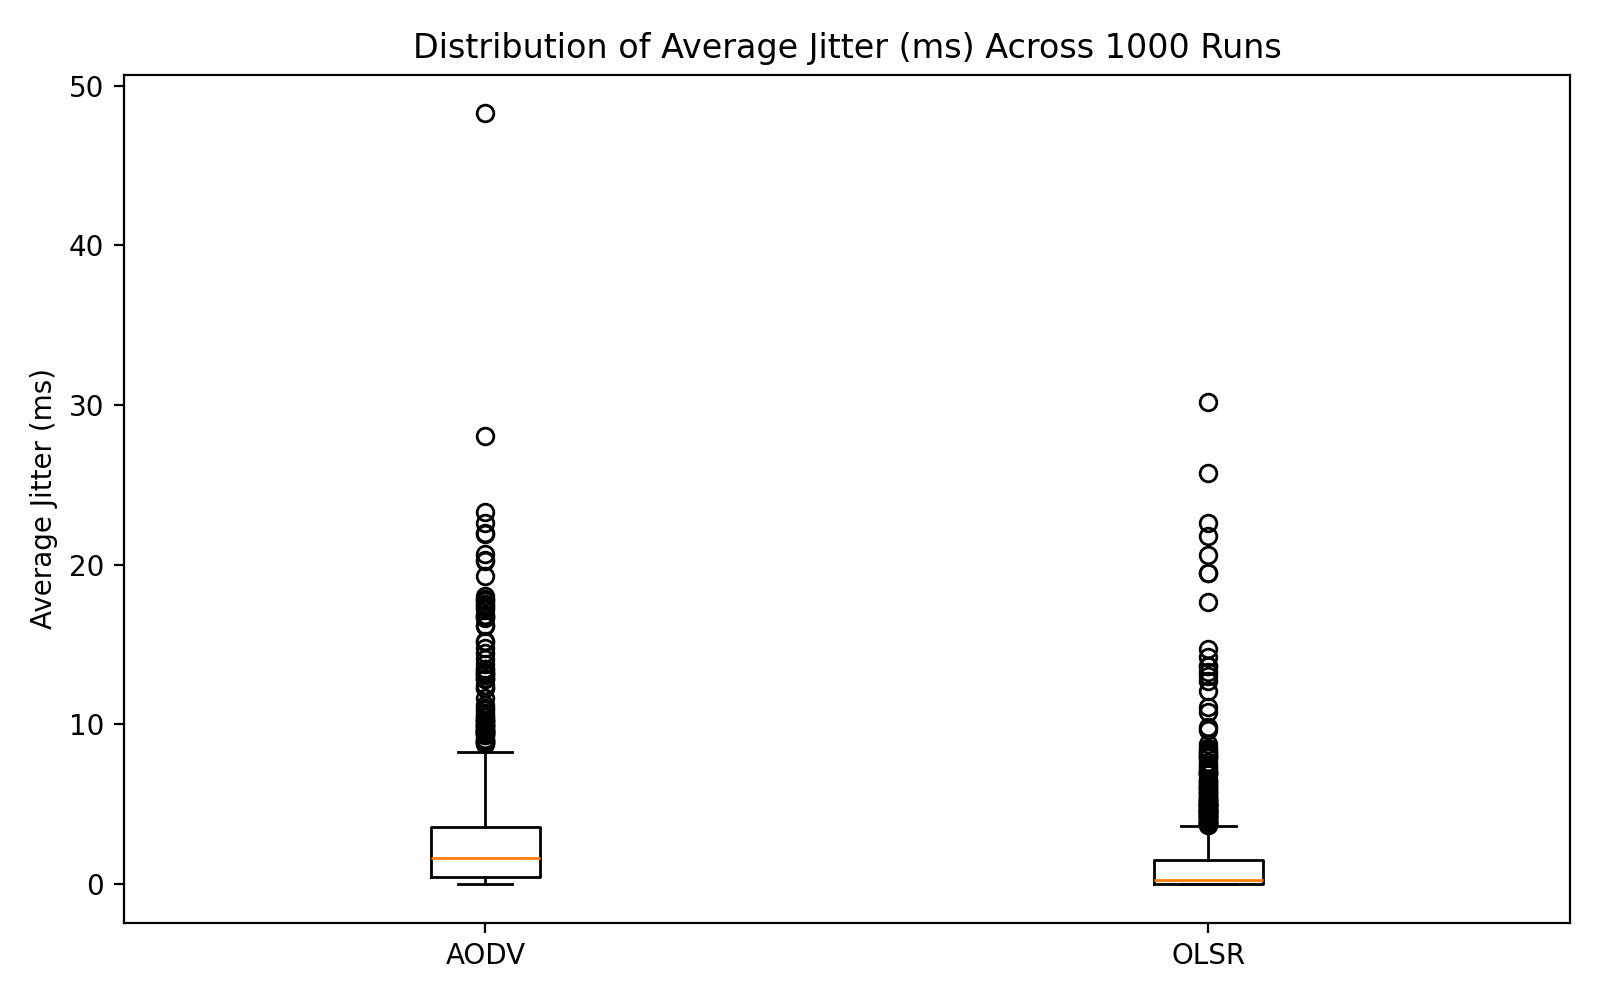
\includegraphics[width=\textwidth]{figures/boxplot_avg_jitter_ms.png}
    \caption{Average jitter}
    \label{fig:app-box-jitter}
\end{subfigure}
\caption{Boxplot comparison of delay and jitter across repeated runs.}
\label{fig:app-box-2}
\end{figure}

\begin{figure}[htbp]
\centering
\begin{subfigure}[t]{0.48\textwidth}
    \centering
    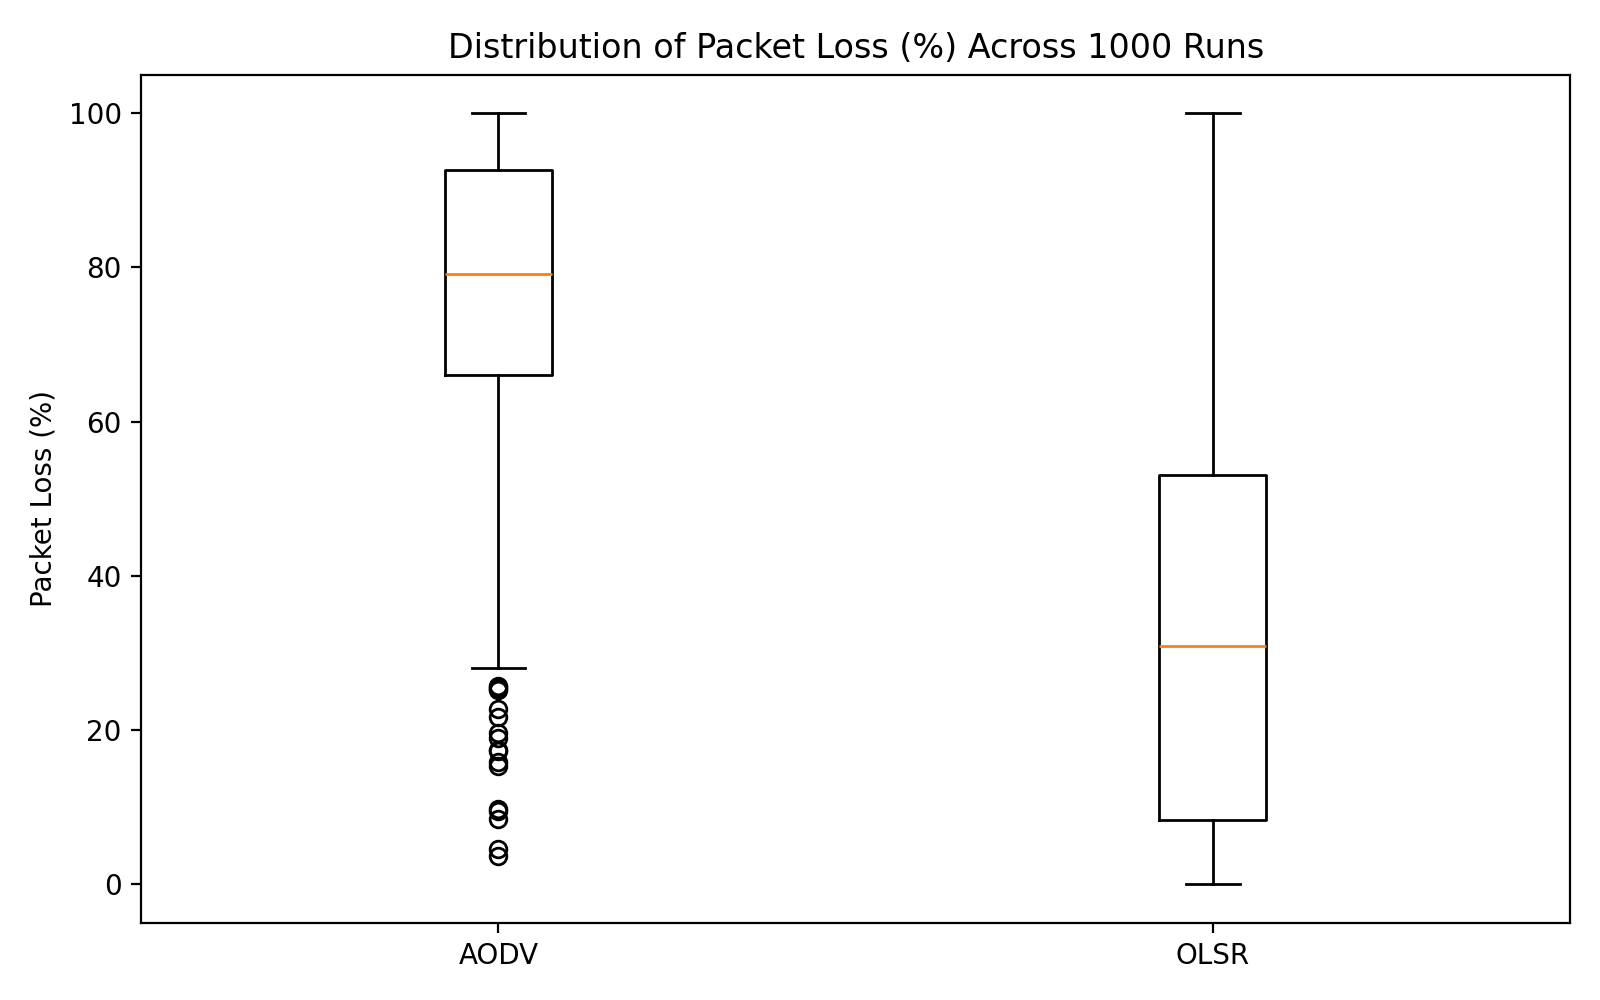
\includegraphics[width=\textwidth]{figures/boxplot_loss_percent.png}
    \caption{Packet loss}
    \label{fig:app-box-loss}
\end{subfigure}
\hfill
\begin{subfigure}[t]{0.48\textwidth}
    \centering
    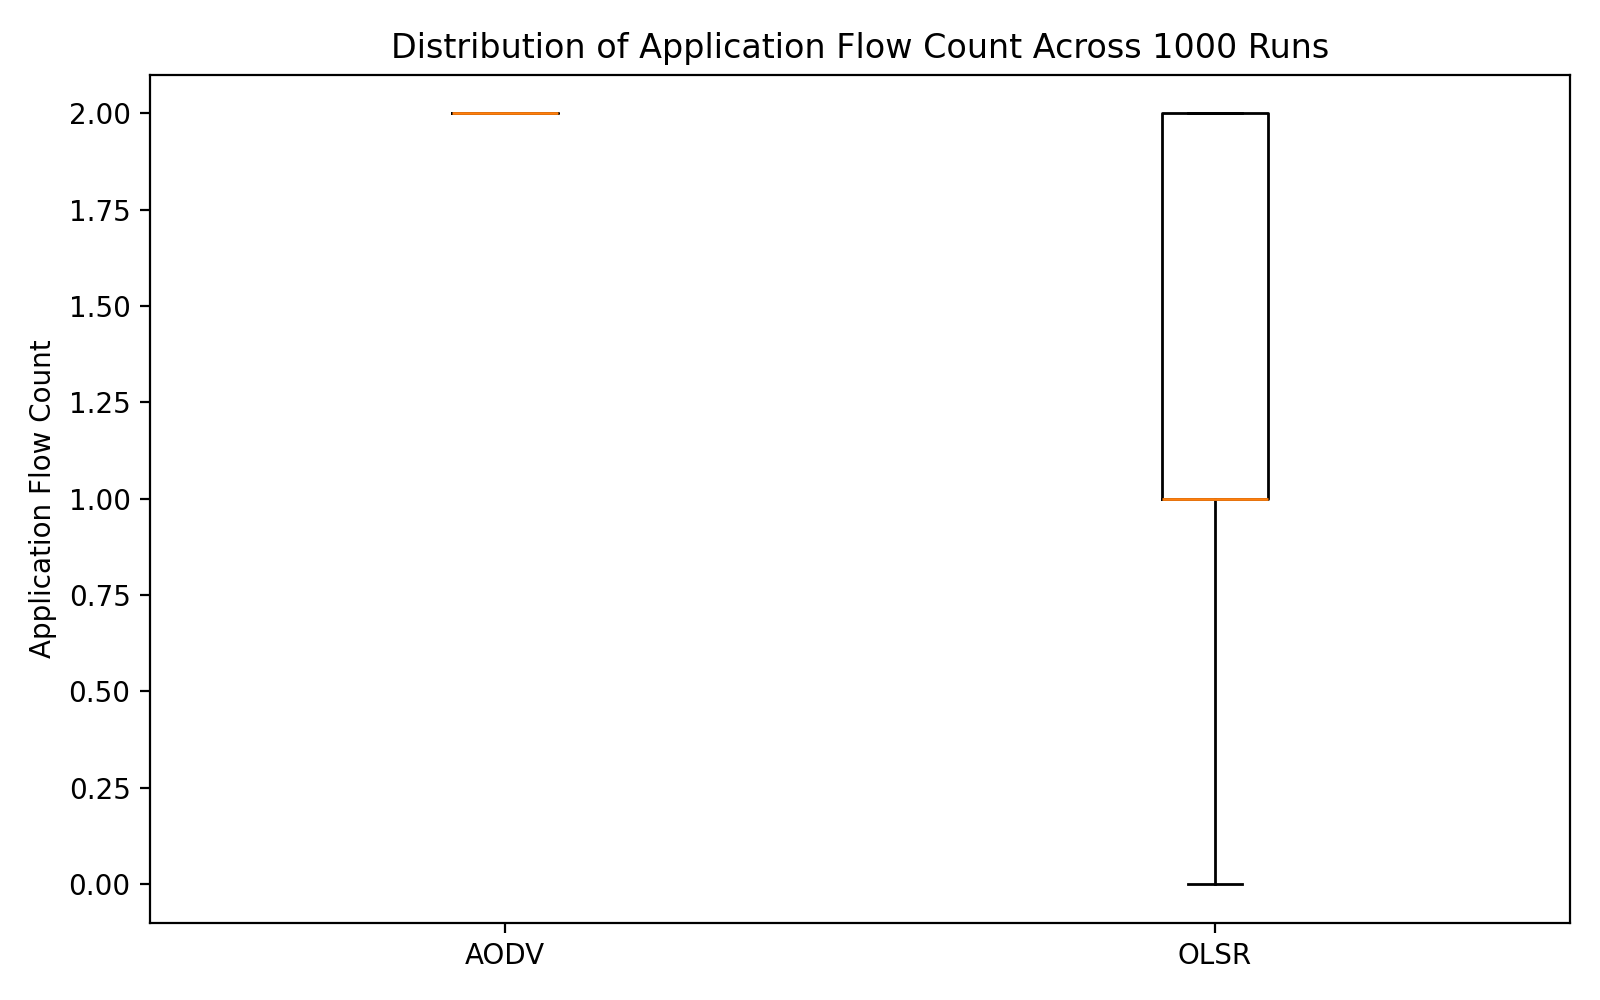
\includegraphics[width=\textwidth]{figures/boxplot_application_flow_count.png}
    \caption{Application-flow count}
    \label{fig:app-box-flowcount}
\end{subfigure}
\caption{Boxplot comparison of packet loss and application-flow count across repeated runs.}
\label{fig:app-box-3}
\end{figure}

\subsection{Histograms}

The histograms provide a frequency-based view of the repeated-run results. Unlike the boxplots, they show how values are distributed across the run set and therefore help illustrate whether the observed protocol behaviour is tightly clustered or broadly spread.

\begin{figure}[htbp]
\centering
\begin{subfigure}[t]{0.48\textwidth}
    \centering
    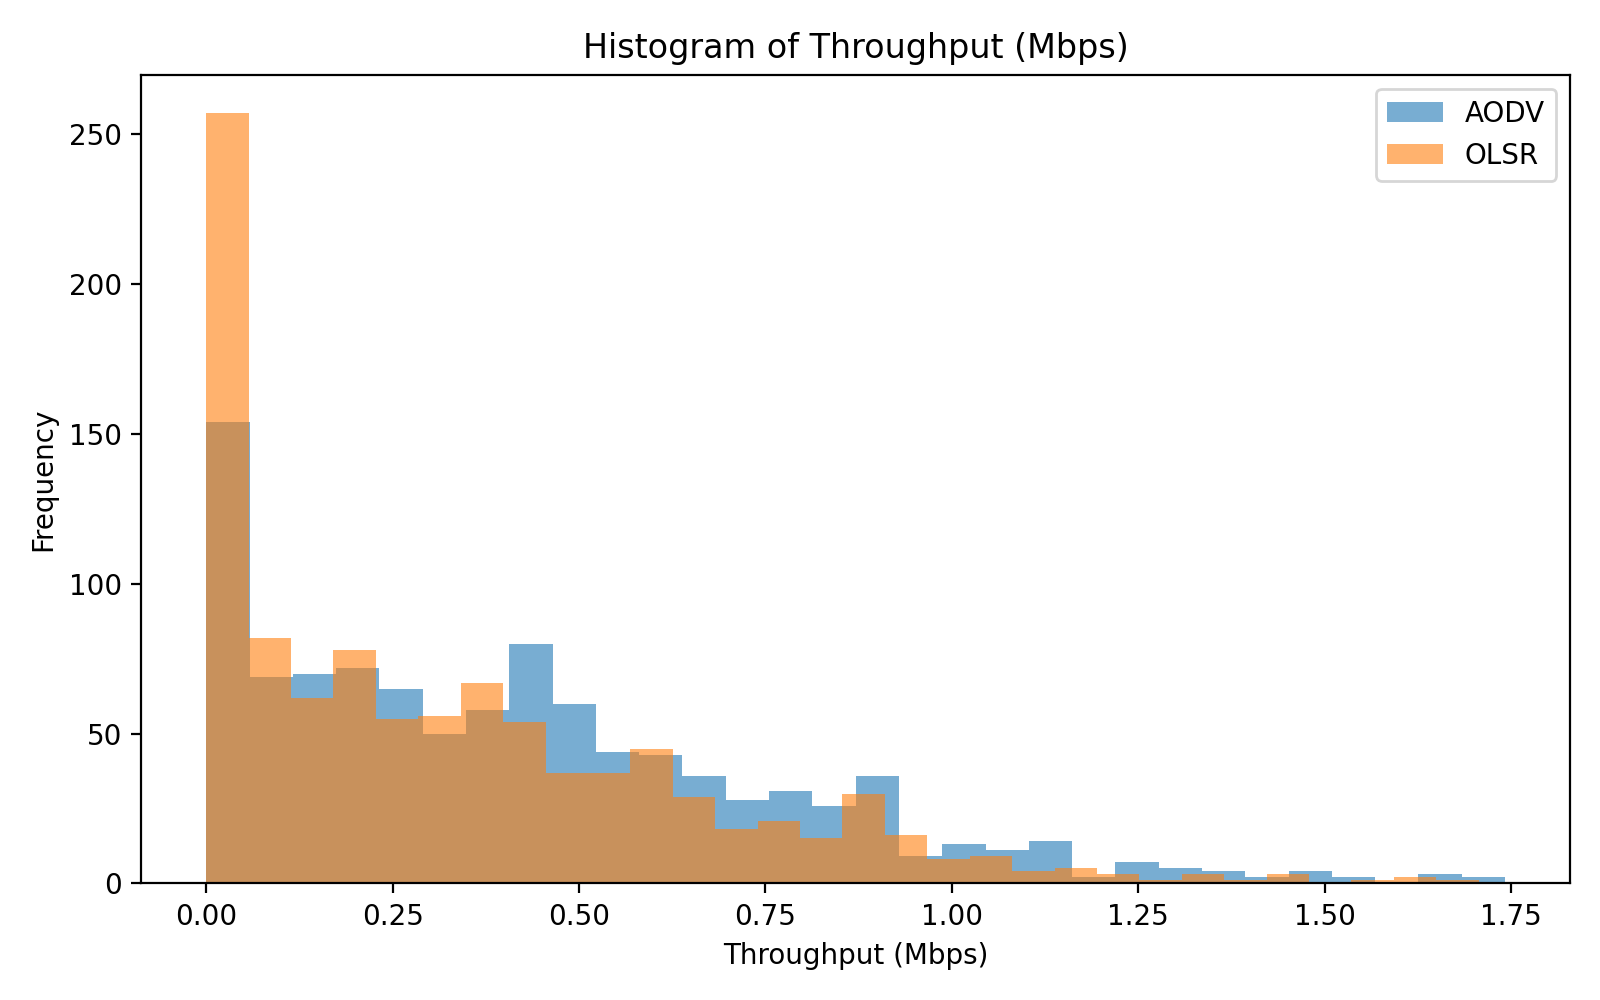
\includegraphics[width=\textwidth]{figures/hist_throughput_mbps.png}
    \caption{Throughput}
    \label{fig:app-hist-throughput}
\end{subfigure}
\hfill
\begin{subfigure}[t]{0.48\textwidth}
    \centering
    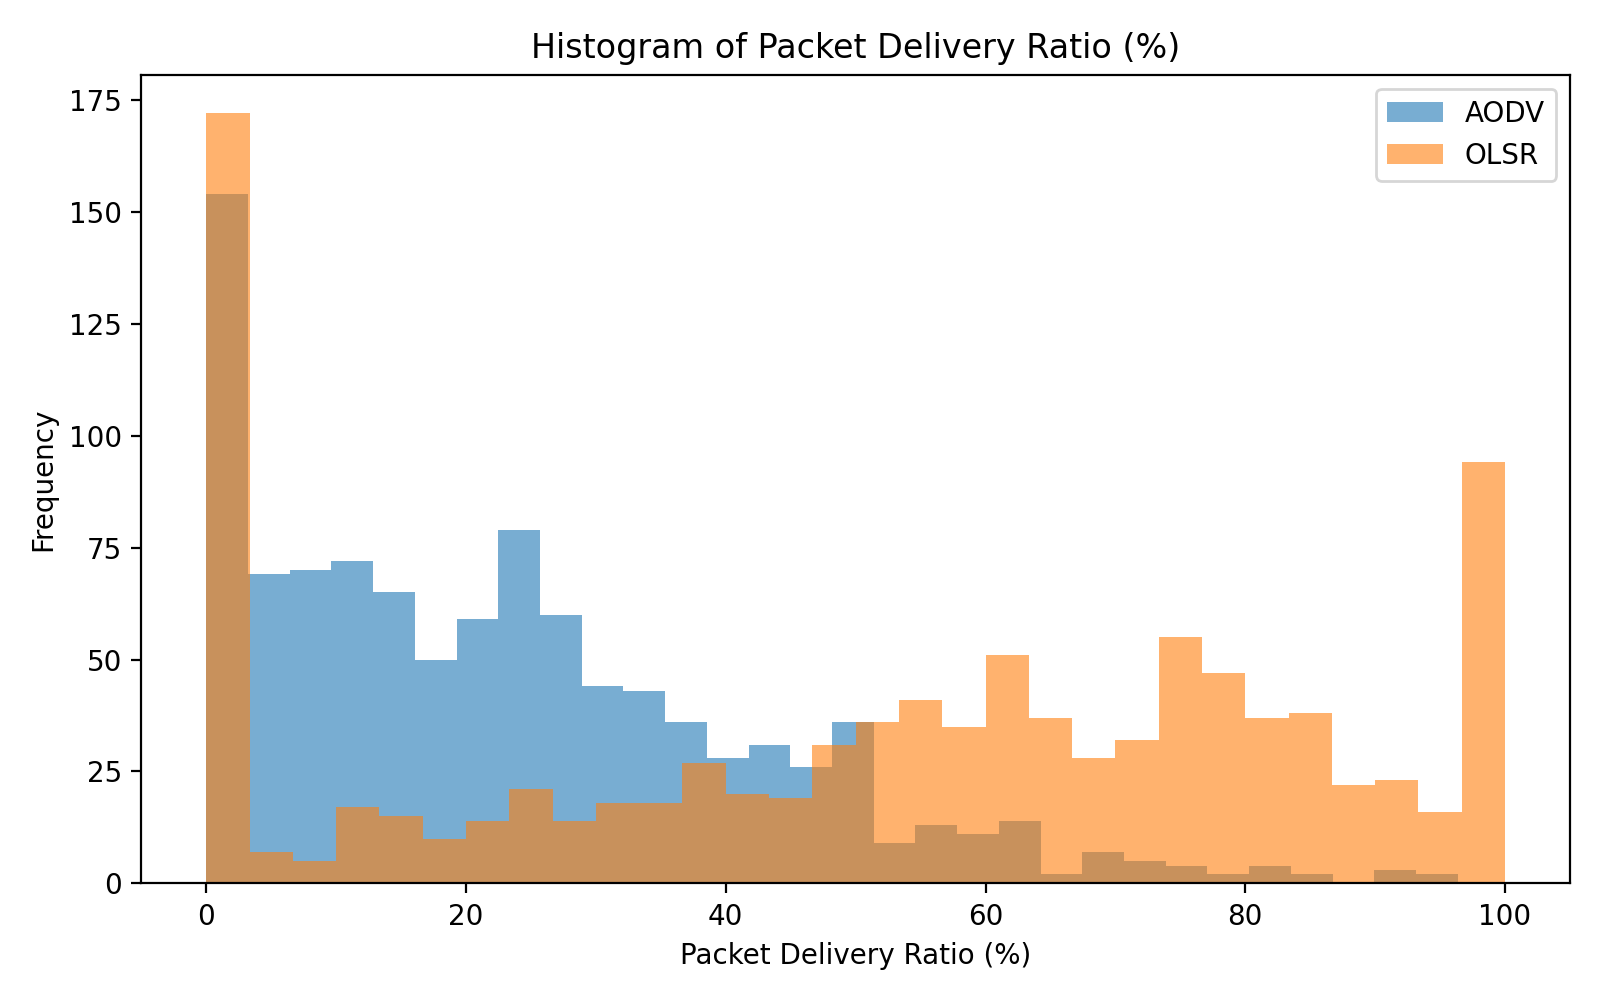
\includegraphics[width=\textwidth]{figures/hist_pdr_percent.png}
    \caption{Packet delivery ratio}
    \label{fig:app-hist-pdr}
\end{subfigure}
\caption{Histogram comparison of throughput and packet delivery ratio across repeated runs.}
\label{fig:app-hist-1}
\end{figure}

\begin{figure}[htbp]
\centering
\begin{subfigure}[t]{0.48\textwidth}
    \centering
    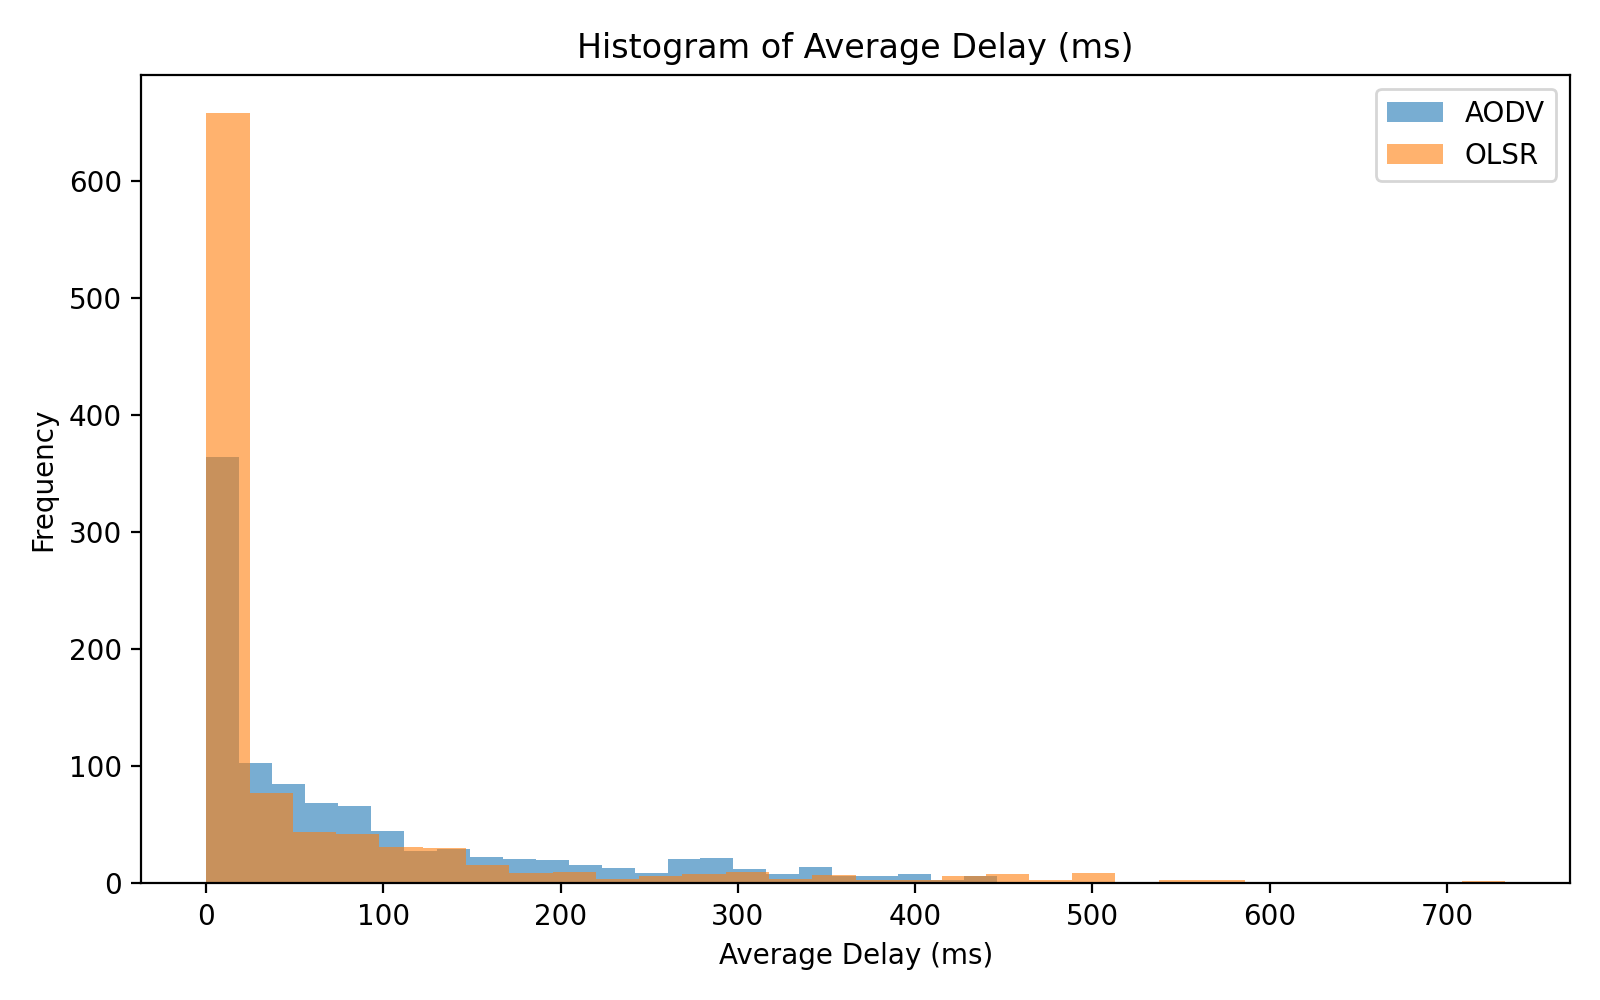
\includegraphics[width=\textwidth]{figures/hist_avg_delay_ms.png}
    \caption{Average delay}
    \label{fig:app-hist-delay}
\end{subfigure}
\hfill
\begin{subfigure}[t]{0.48\textwidth}
    \centering
    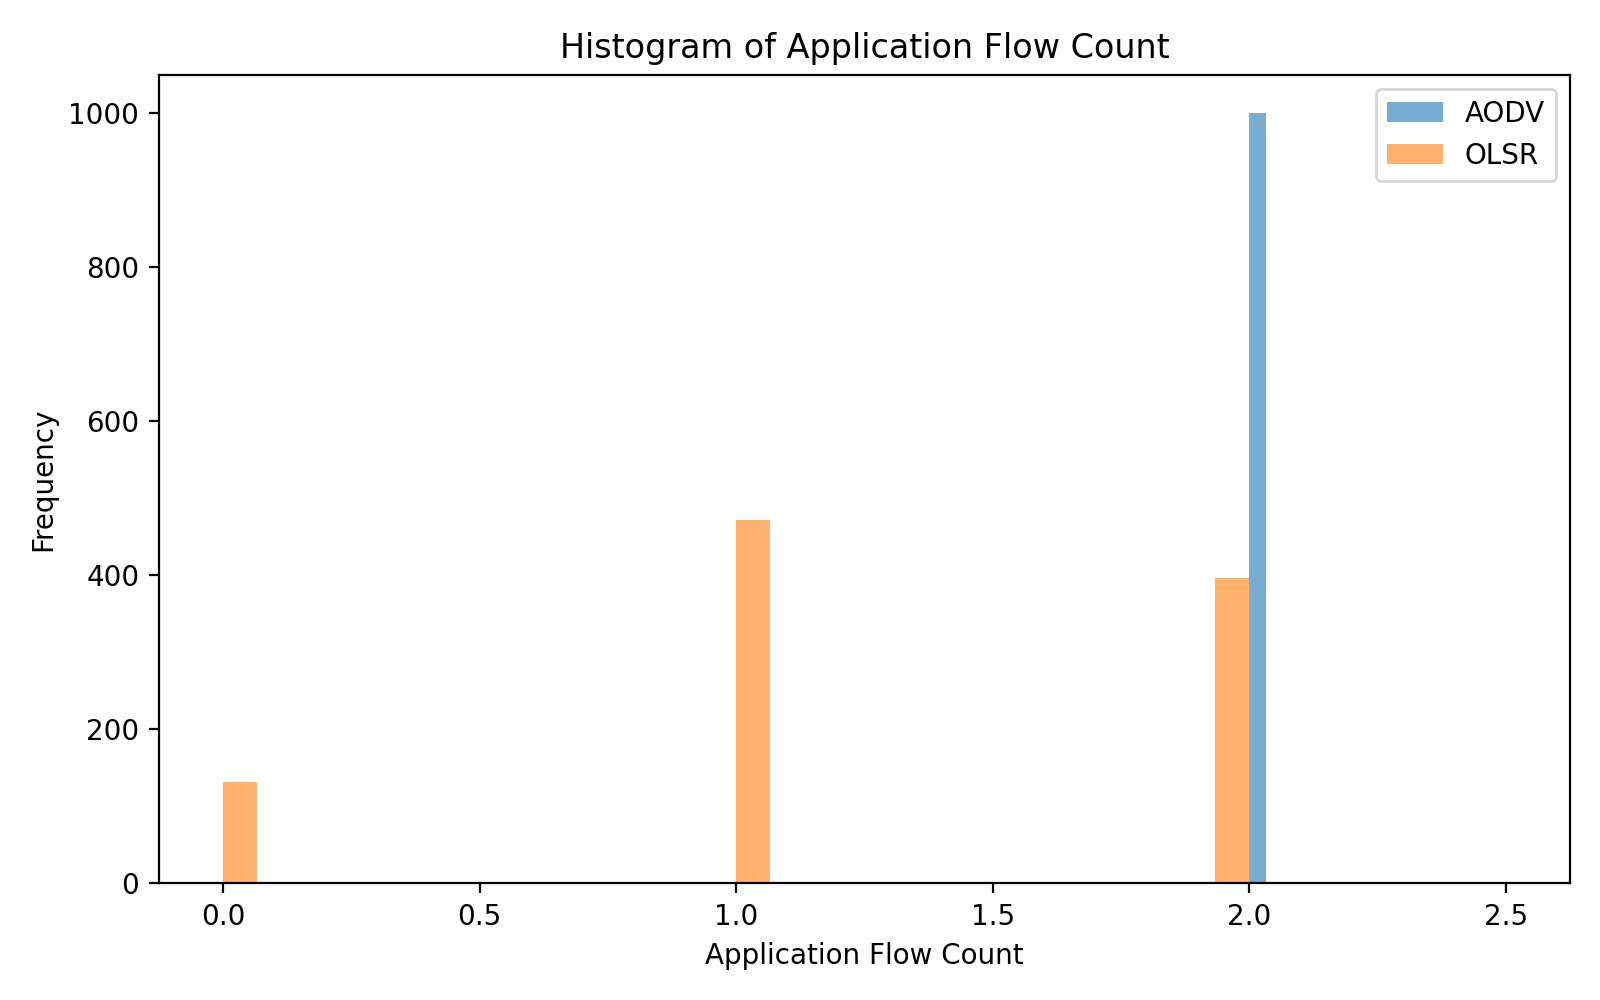
\includegraphics[width=\textwidth]{figures/hist_application_flow_count.png}
    \caption{Application-flow count}
    \label{fig:app-hist-flowcount}
\end{subfigure}
\caption{Histogram comparison of average delay and application-flow count across repeated runs.}
\label{fig:app-hist-2}
\end{figure}

\subsection{Error-Bar Plots}

The error-bar plots summarise the repeated-run metrics in terms of mean value and standard deviation. Their purpose is to show not only the average performance level of each protocol, but also the degree of variability associated with that average. This helps clarify whether a stronger aggregate mean is accompanied by relatively stable behaviour or by wider dispersion across runs.

\begin{figure}[htbp]
\centering
\begin{subfigure}[t]{0.48\textwidth}
    \centering
    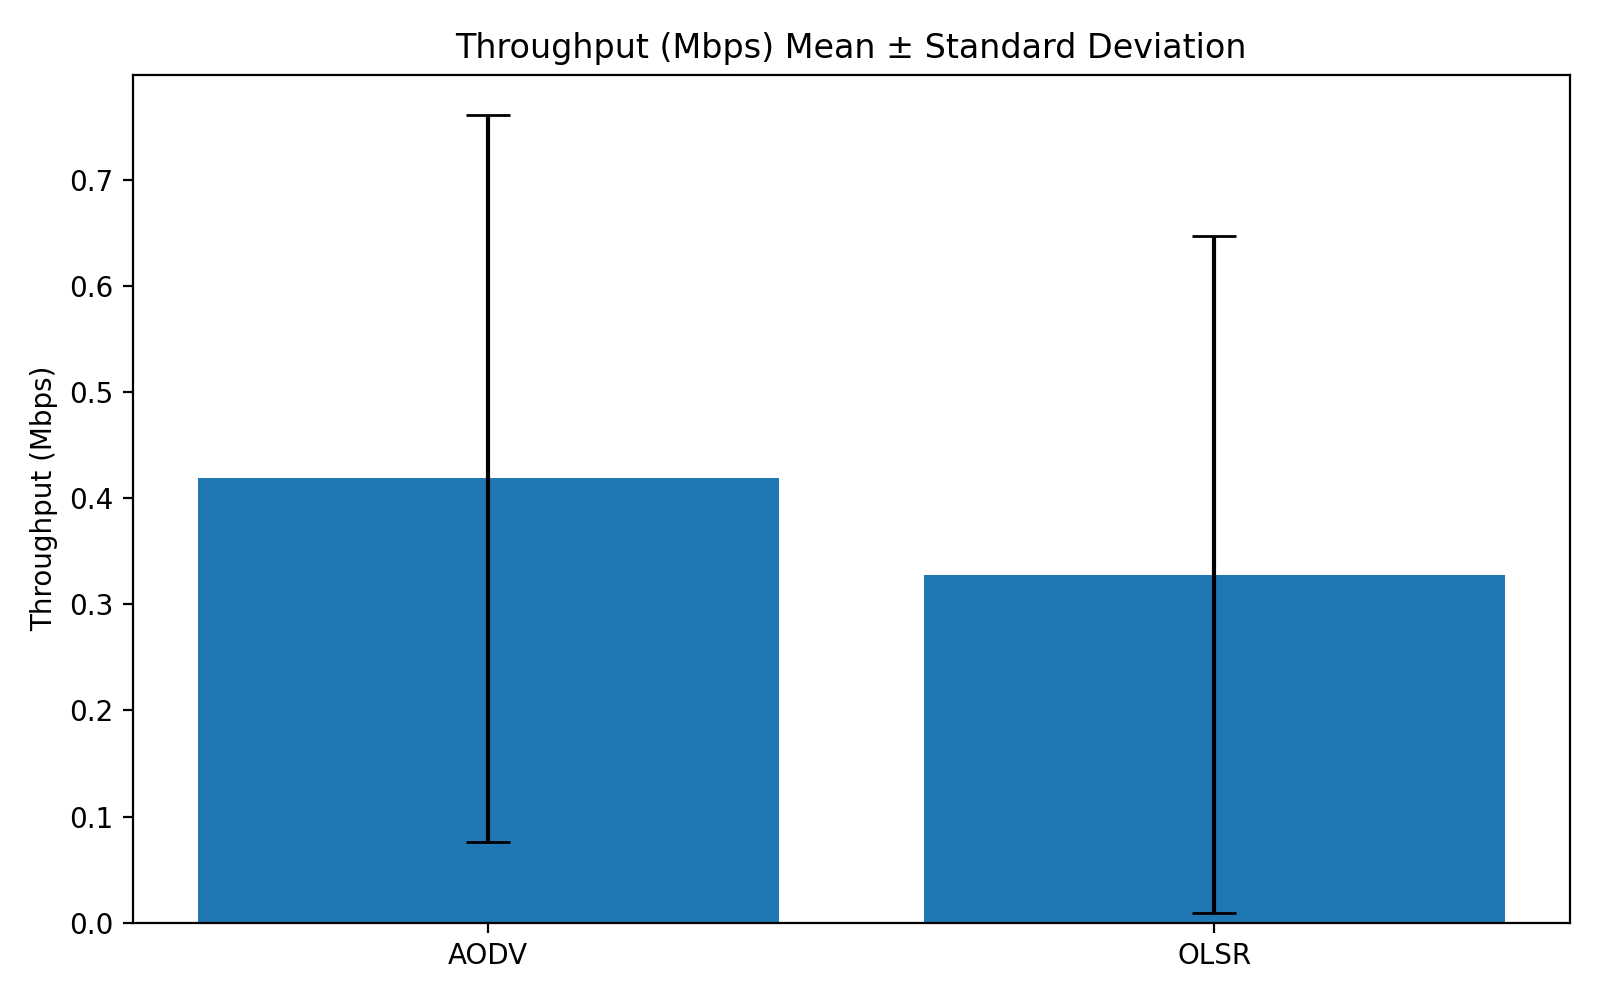
\includegraphics[width=\textwidth]{figures/errorbar_throughput_mbps.png}
    \caption{Throughput}
    \label{fig:app-error-throughput}
\end{subfigure}
\hfill
\begin{subfigure}[t]{0.48\textwidth}
    \centering
    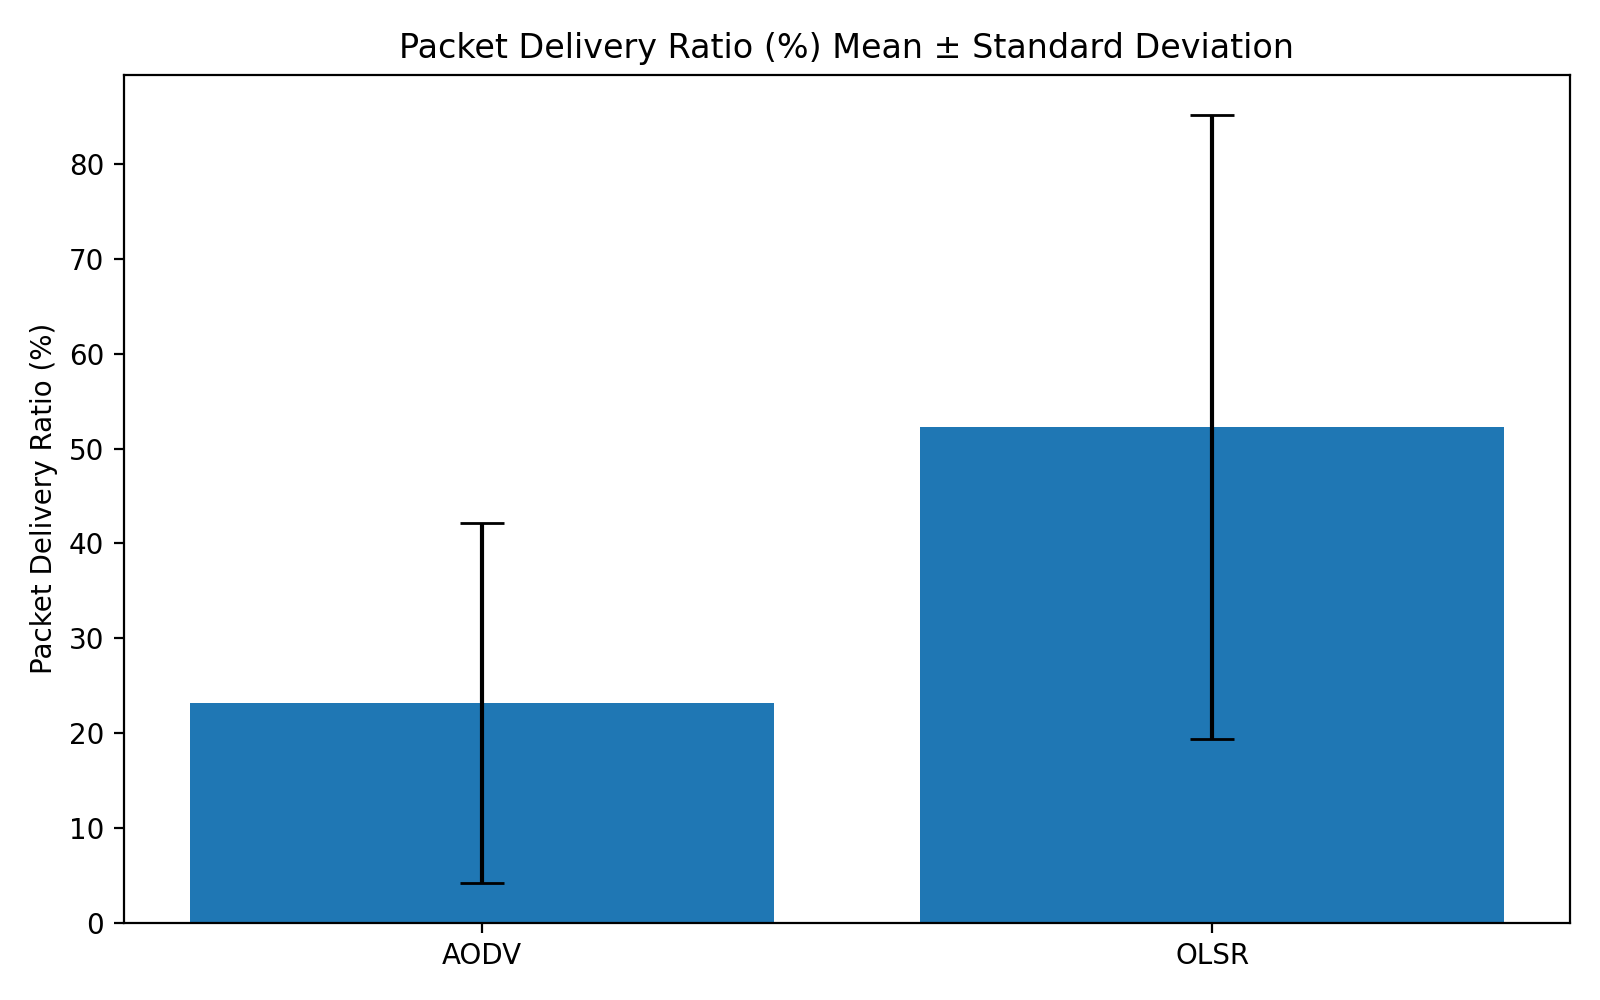
\includegraphics[width=\textwidth]{figures/errorbar_pdr_percent.png}
    \caption{Packet delivery ratio}
    \label{fig:app-error-pdr}
\end{subfigure}
\caption{Error-bar comparison of throughput and packet delivery ratio across repeated runs.}
\label{fig:app-error-1}
\end{figure}

\begin{figure}[htbp]
\centering
\begin{subfigure}[t]{0.48\textwidth}
    \centering
    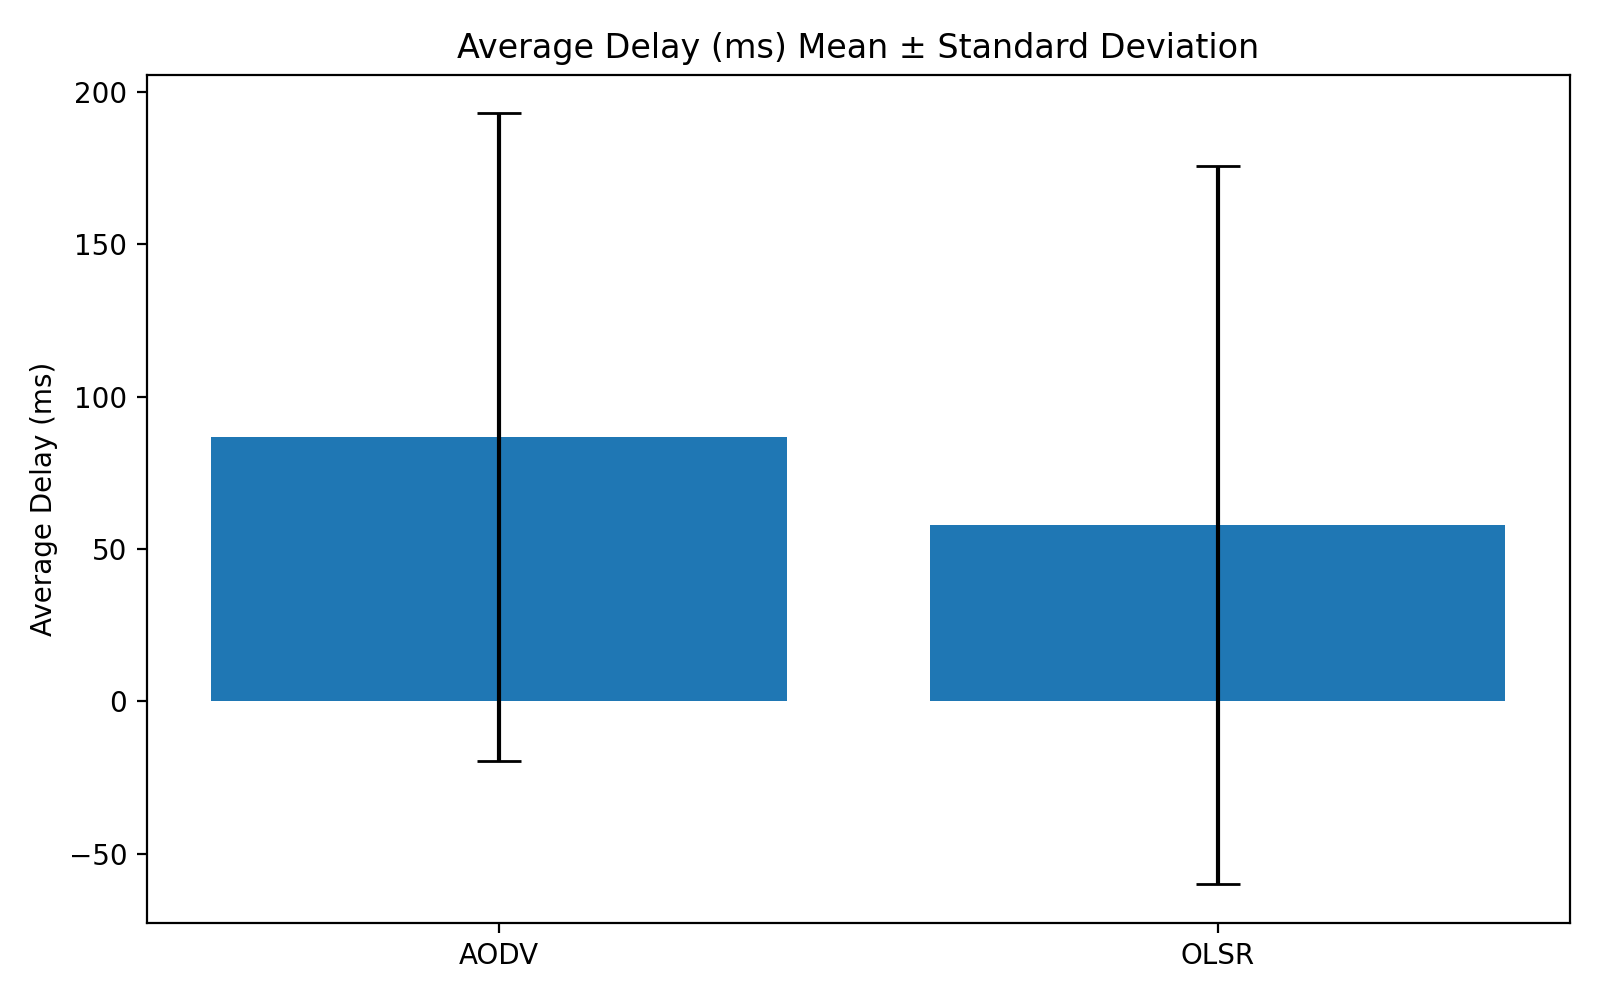
\includegraphics[width=\textwidth]{figures/errorbar_avg_delay_ms.png}
    \caption{Average delay}
    \label{fig:app-error-delay}
\end{subfigure}
\hfill
\begin{subfigure}[t]{0.48\textwidth}
    \centering
    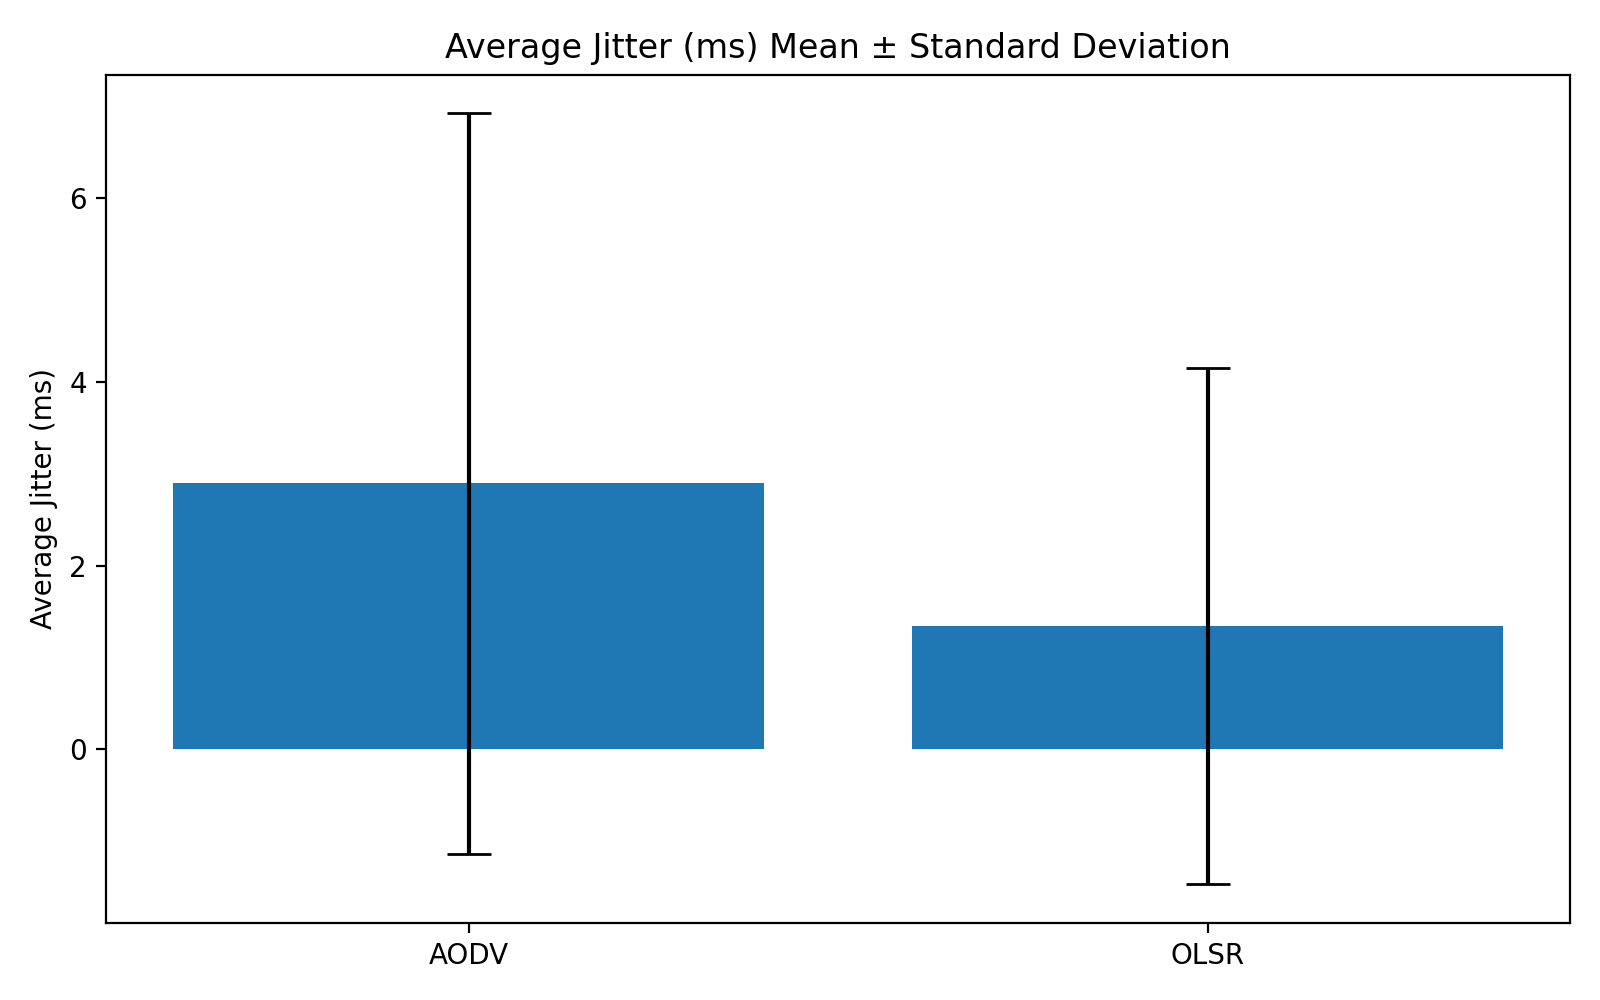
\includegraphics[width=\textwidth]{figures/errorbar_avg_jitter_ms.png}
    \caption{Average jitter}
    \label{fig:app-error-jitter}
\end{subfigure}
\caption{Error-bar comparison of delay and jitter across repeated runs.}
\label{fig:app-error-2}
\end{figure}

These plots supplement the aggregate results by showing that the comparison is not based on mean values alone, but also on the consistency of each metric across repeated simulation runs.

\subsection{Run-Order Line Plots}

The run-order line plots present the behaviour of selected metrics across the full sequence of repeated runs. Unlike the boxplots, histograms, and error-bar plots, which summarise distributions, these figures preserve run ordering and therefore help reveal whether performance fluctuated noticeably over the sequence of executions. They are particularly useful for identifying visible instability, persistence, or irregularity in the repeated-run outputs.

\begin{figure}[htbp]
\centering
\begin{subfigure}[t]{0.65\textwidth}
    \centering
    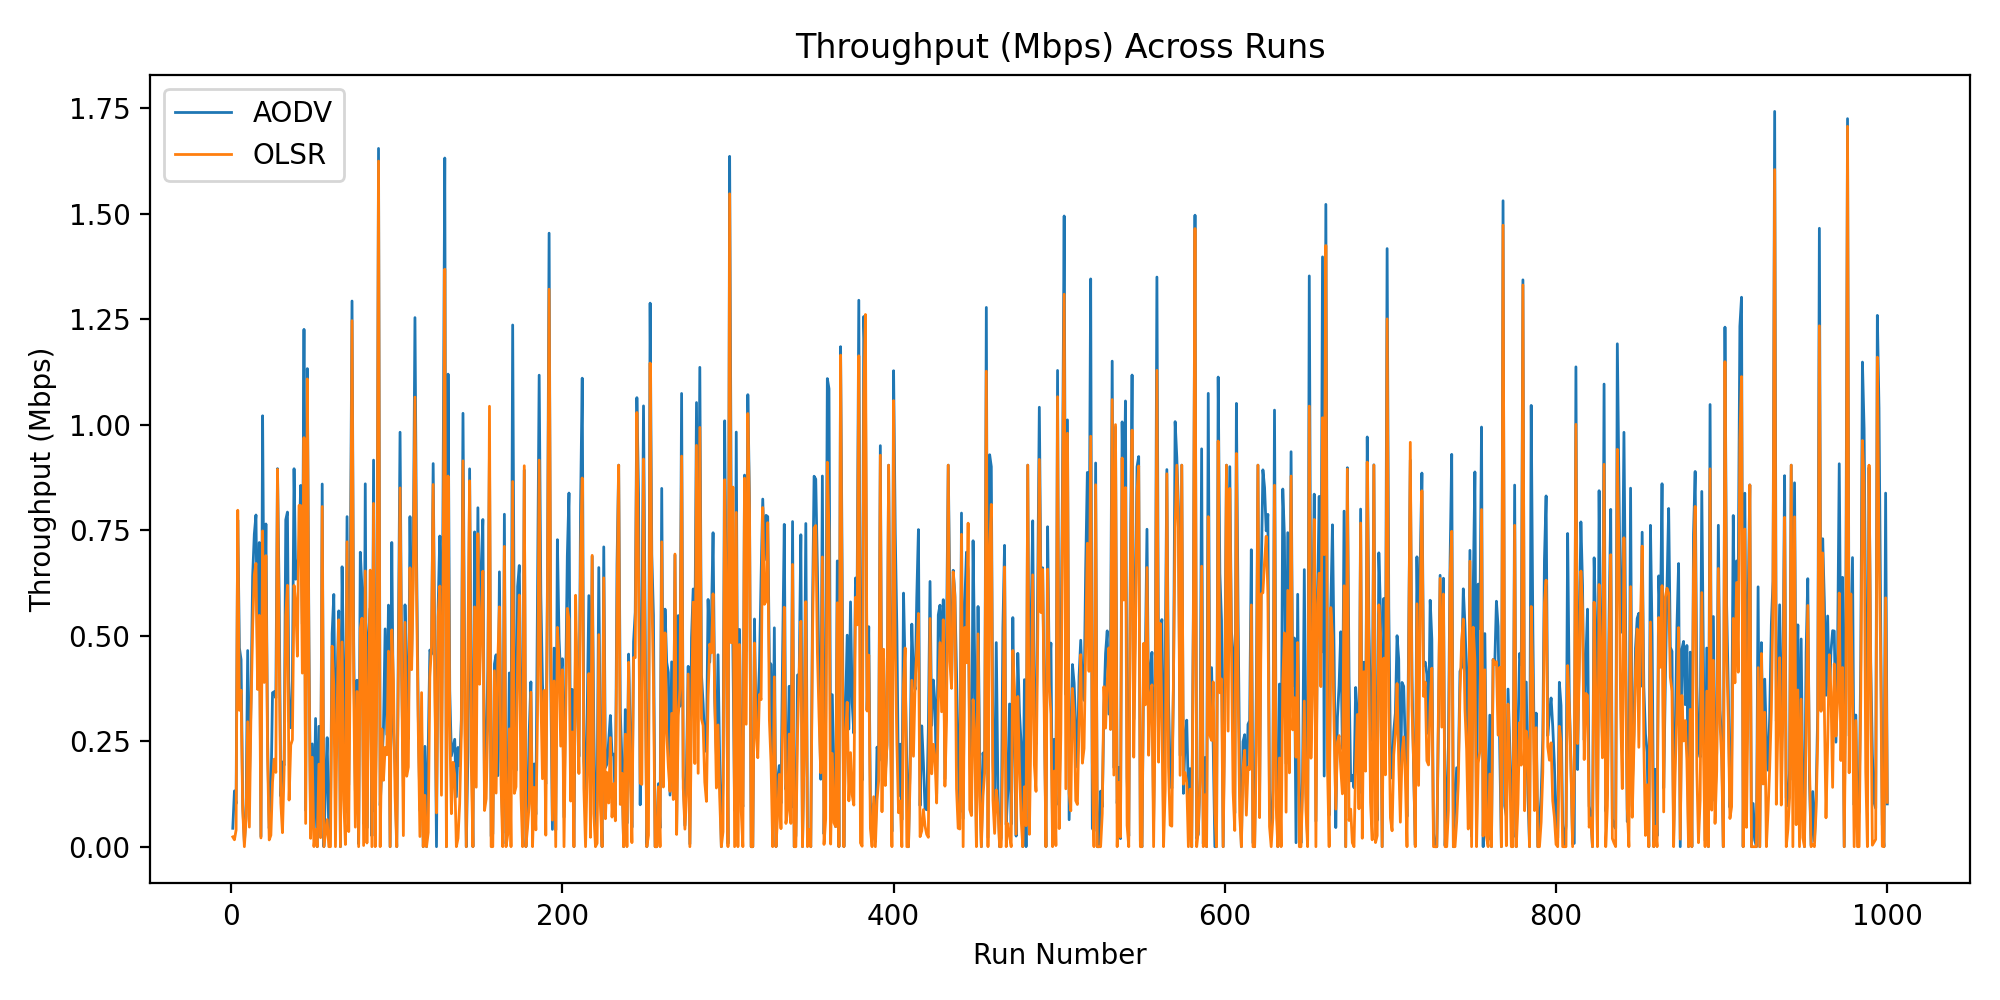
\includegraphics[width=\textwidth]{figures/line_throughput_mbps.png}
    \caption{Throughput}
    \label{fig:app-line-throughput}
\end{subfigure}
\hfill
\begin{subfigure}[t]{0.65\textwidth}
    \centering
    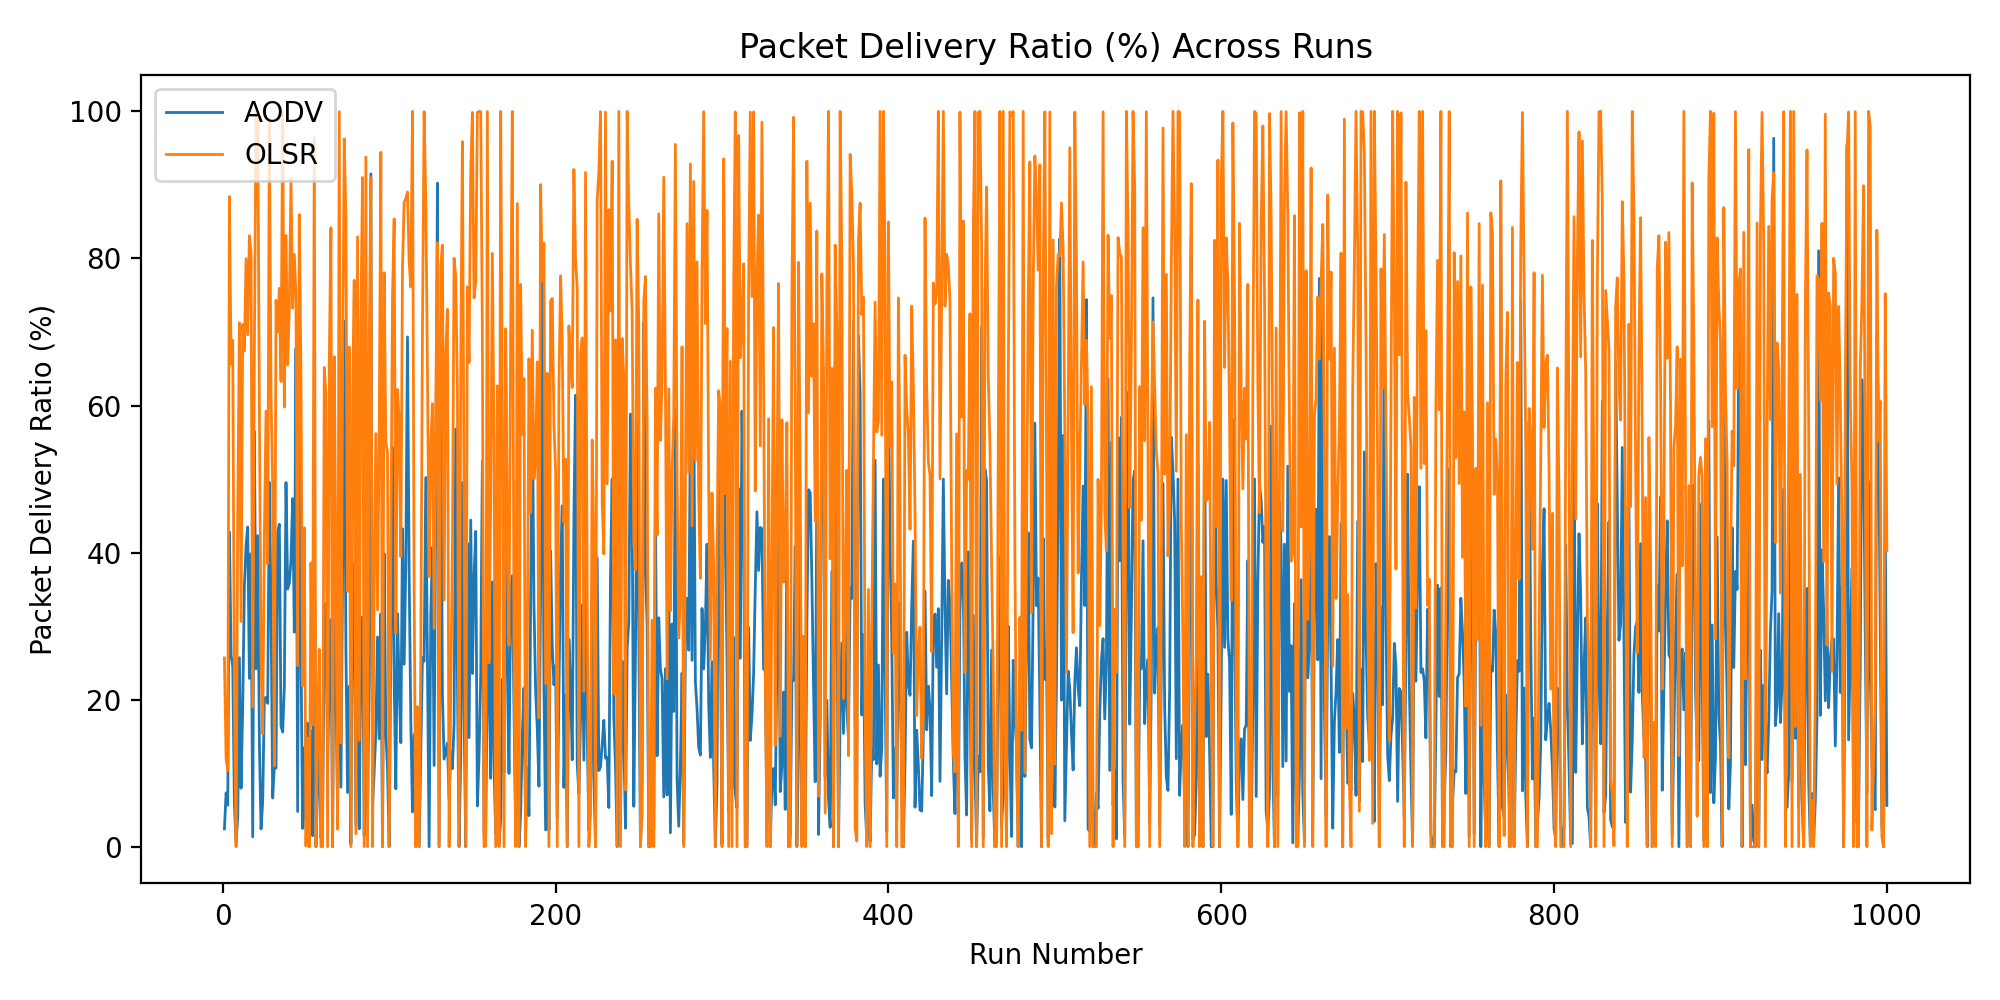
\includegraphics[width=\textwidth]{figures/line_pdr_percent.png}
    \caption{Packet delivery ratio}
    \label{fig:app-line-pdr}
\end{subfigure}
\caption{Run-order line comparison of throughput and packet delivery ratio across repeated runs.}
\label{fig:app-line-1}
\end{figure}

\begin{figure}[htbp]
\centering
\begin{subfigure}[t]{0.65\textwidth}
    \centering
    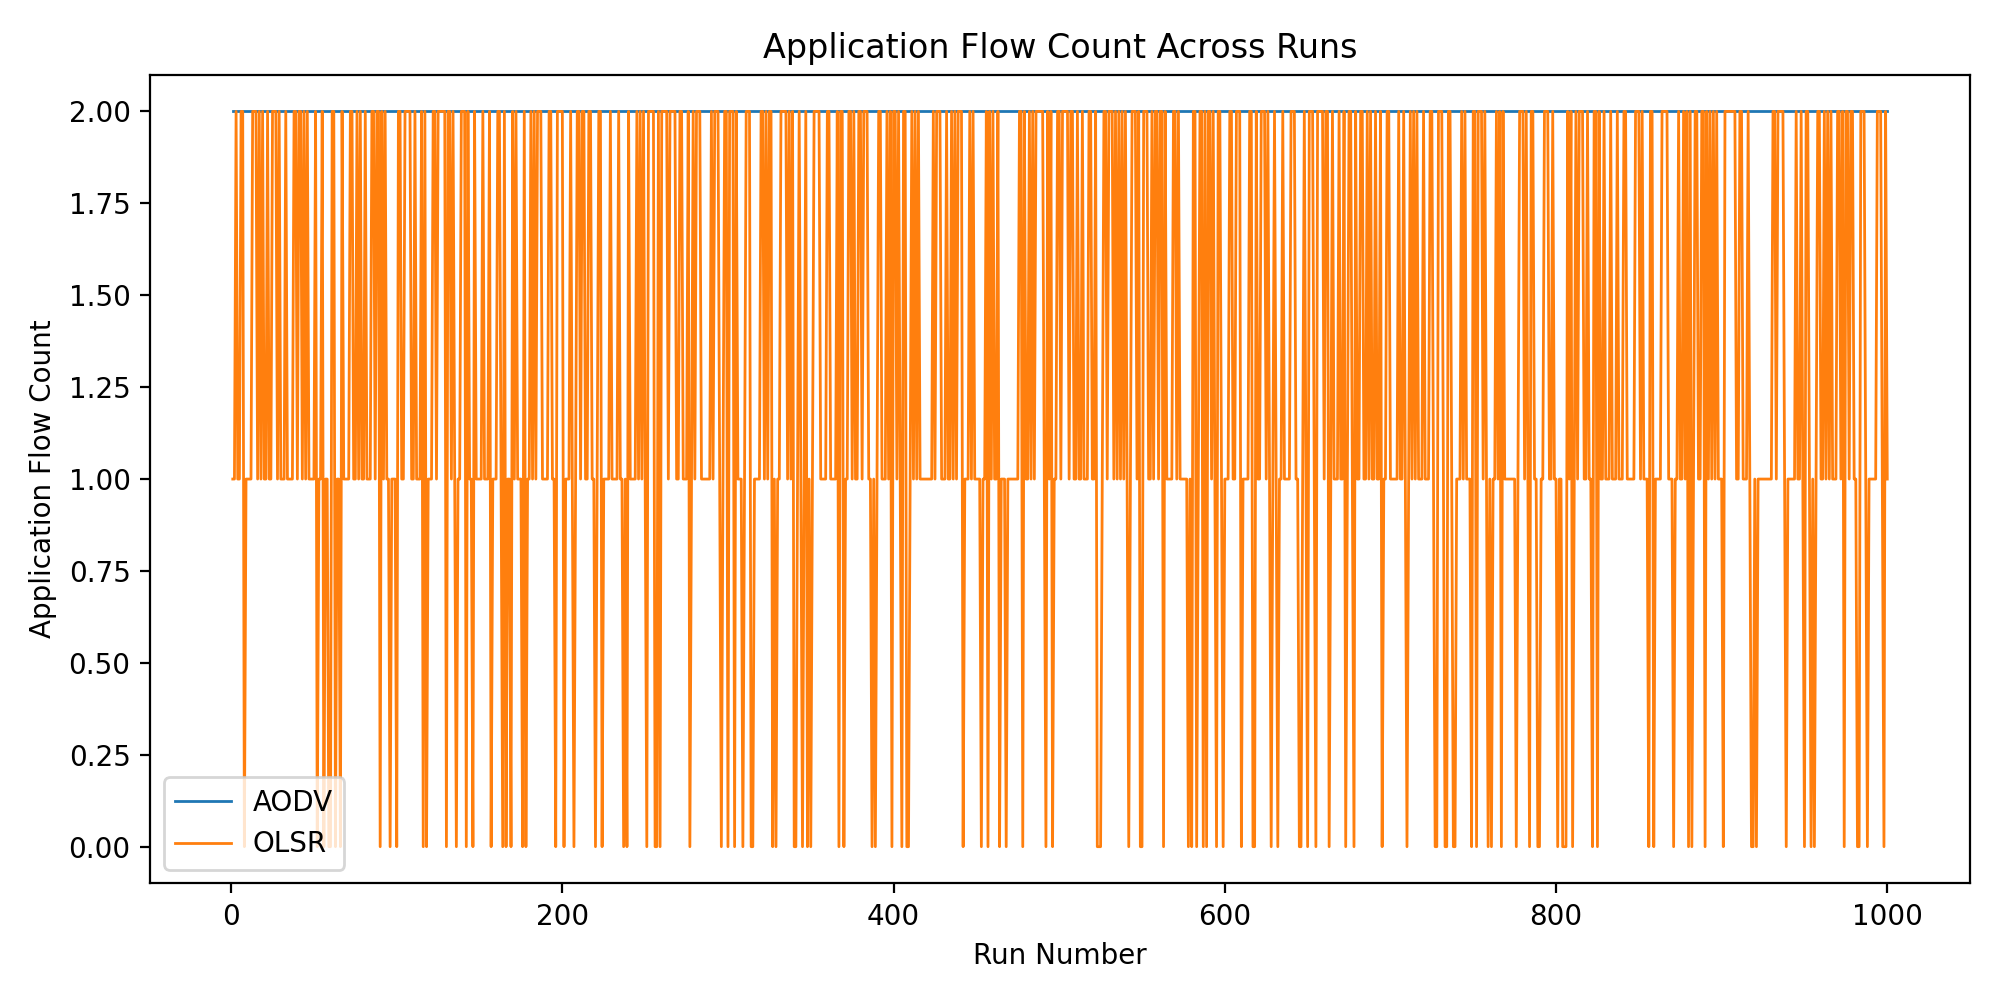
\includegraphics[width=\textwidth]{figures/line_application_flow_count.png}
    \caption{Application-flow count}
    \label{fig:app-line-flowcount}
\end{subfigure}
\caption{Run-order line plot of application-flow count across repeated runs.}
\label{fig:app-line-2}
\end{figure}

Taken together, the line plots reinforce the distribution-based analysis by showing how metric behaviour varied across the repeated execution sequence rather than only in aggregate form.

\FloatBarrier
\section{Supporting Scripts}
\label{app:scripts}

This section documents the scripts used to automate the experiment workflow. These scripts handled repeated simulation execution, FlowMonitor parsing, graph generation, CSV export, and AI-assisted interpretation. Their inclusion in the appendix provides direct evidence that the study followed a reproducible processing pipeline rather than relying on manual inspection alone.

Table~\ref{tab:scripts} provides an overview of the main scripts and their functions within the workflow.

\begin{table}[htbp]
\centering
\caption{Supporting scripts used in the experiment workflow}
\label{tab:scripts}
\begin{tabular}{lp{9cm}}
\toprule
\textbf{Script} & \textbf{Purpose} \\
\midrule
\texttt{run\_batch.py} & Executes repeated NS-3 runs for both AODV and OLSR using the configured 20-node, \(300 \times 300\) m, UDP CBR scenario. \\
\texttt{parse\_flowmonitor.py} & Parses FlowMonitor XML outputs, filters the experiment application flows, and computes throughput, packet delivery ratio, loss, delay, and jitter. \\
\texttt{make\_graphs.py} & Generates the main comparison graphs used in the Results section. \\
\texttt{make\_distribution\_graphs.py} & Produces boxplots, histograms, line plots, and error-bar plots for repeated-run distribution analysis. \\
\texttt{json\_to\_csv.py} & Exports per-run and summary metrics into CSV format for reporting and comparison. \\
\texttt{ask\_ai.py} & Sends final summary metrics for AI-assisted interpretation and stores the structured output. \\
\bottomrule
\end{tabular}
\end{table}

The excerpts below illustrate the most important parts of the automated workflow, beginning with repeated simulation execution, followed by metric extraction, distribution-based graph generation, CSV export, and the constrained AI prompt used for interpretation.

\begin{lstlisting}[language=Python, caption={Excerpt from \texttt{run\_batch.py} showing repeated execution settings}]
PROTOCOLS = ["AODV", "OLSR"]
RUNS = range(1, 1001)

COMMON_ARGS = {
    "nFlows": 2,
    "areaX": 300,
    "areaY": 300,
    "minSpeed": 1,
    "maxSpeed": 3,
    "pauseTime": 2,
    "simTime": 70,
    "serverStartTime": 1,
    "clientStartTime": 10,
    "packetSize": 512,
    "dataRate": "1Mbps",
}
\end{lstlisting}

\begin{lstlisting}[language=Python, caption={Excerpt from \texttt{parse\_flowmonitor.py} showing metric computation}]
throughput_bps = (rx_bytes * 8) / sim_time if sim_time > 0 else 0.0
throughput_mbps = throughput_bps / 1_000_000

pdr_percent = (rx_packets / tx_packets * 100) if tx_packets > 0 else 0.0
loss_percent = ((tx_packets - rx_packets) / tx_packets * 100) if tx_packets > 0 else 0.0

avg_delay_s = (delay_sum_s / rx_packets) if rx_packets > 0 else 0.0
avg_delay_ms = avg_delay_s * 1000

avg_jitter_s = (jitter_sum_s / rx_packets) if rx_packets > 0 else 0.0
avg_jitter_ms = avg_jitter_s * 1000
\end{lstlisting}

\begin{lstlisting}[language=Python, caption={Excerpt from \texttt{make\_distribution\_graphs.py} showing repeated-run chart generation}]
boxplot_metrics = [
    ("throughput_mbps", "Throughput (Mbps)"),
    ("pdr_percent", "Packet Delivery Ratio (%)"),
    ("loss_percent", "Packet Loss (%)"),
    ("avg_delay_ms", "Average Delay (ms)"),
    ("avg_jitter_ms", "Average Jitter (ms)"),
    ("application_flow_count", "Application Flow Count"),
]
\end{lstlisting}

\begin{lstlisting}[language=Python, caption={Excerpt from \texttt{json\_to\_csv.py} showing summary CSV export}]
summary_rows.append({
    "protocol": protocol,
    "runs": s.get("runs"),
    "avg_application_flow_count": s.get("avg_application_flow_count"),
    "avg_throughput_mbps": s.get("avg_throughput_mbps"),
    "avg_pdr_percent": s.get("avg_pdr_percent"),
    "avg_loss_percent": s.get("avg_loss_percent"),
    "avg_delay_ms": s.get("avg_delay_ms"),
    "avg_jitter_ms": s.get("avg_jitter_ms"),
})
\end{lstlisting}

\begin{lstlisting}[language=Python, caption={Excerpt from \texttt{ask\_ai.py} showing the constrained AI analysis prompt}]
You are analyzing final NS-3 MANET experiment results.
Use only the supplied numbers.
Do not invent values.
Be academically careful.
If the comparison is affected by unequal active flow counts, state that clearly.
\end{lstlisting}

\FloatBarrier
\section{CSV Output Summaries}
\label{app:csv}

This section provides representative extracts from the CSV outputs generated during the analysis stage. Two CSV files were created: one containing per-run metrics and another containing aggregate protocol-level summary metrics. These outputs formed the basis of the summary table and the graphs presented in the main Results section.

Table~\ref{tab:csv-fields} lists the most important fields exported to the summary CSV file and shows how the aggregate values used in the report were structured.

\begin{table}[htbp]
\centering
\caption{Key fields exported to the summary CSV file}
\label{tab:csv-fields}
\begin{tabular}{ll}
\toprule
\textbf{Field} & \textbf{Description} \\
\midrule
\texttt{protocol} & Routing protocol under evaluation \\
\texttt{runs} & Number of simulation runs aggregated \\
\texttt{avg\_application\_flow\_count} & Mean active application-flow count \\
\texttt{avg\_throughput\_mbps} & Mean throughput in Mbps \\
\texttt{avg\_pdr\_percent} & Mean packet delivery ratio \\
\texttt{avg\_loss\_percent} & Mean packet loss percentage \\
\texttt{avg\_delay\_ms} & Mean end-to-end delay in milliseconds \\
\texttt{avg\_jitter\_ms} & Mean jitter in milliseconds \\
\texttt{avg\_tx\_packets} & Mean transmitted packets \\
\texttt{avg\_rx\_packets} & Mean received packets \\
\texttt{avg\_lost\_packets} & Mean lost packets \\
\bottomrule
\end{tabular}
\end{table}

The following excerpts show the structure of both the summary CSV and the per-run CSV.

\begin{lstlisting}[caption={Excerpt from the summary CSV output}]
protocol,runs,avg_application_flow_count,avg_throughput_mbps,avg_pdr_percent,avg_loss_percent,avg_delay_ms,avg_jitter_ms
AODV,1000,2.000,0.4188,23.16,76.84,86.72,2.89
OLSR,1000,1.264,0.3282,52.26,34.54,57.87,1.34
\end{lstlisting}

\begin{lstlisting}[caption={Representative fields from the per-run CSV output}]
protocol,file,application_flow_count,tx_packets,rx_packets,lost_packets,throughput_mbps,pdr_percent,loss_percent,avg_delay_ms,avg_jitter_ms
AODV,final1000_AODV_1.xml,2,...,...,...,...,...,...,...,...
OLSR,final1000_OLSR_1.xml,1,...,...,...,...,...,...,...,...
\end{lstlisting}

\FloatBarrier
\section{AI-Assisted Analysis Evidence}
\label{app:ai}

This section documents the AI-assisted interpretation stage used after metric extraction. The AI workflow was constrained to use only the final measured summary values and was not permitted to invent, alter, or replace the original results. Its role was therefore limited to structured comparison and interpretive support.

Table~\ref{tab:ai-summary} shows the protocol winners identified by the structured AI output across the main comparison criteria.

\begin{table}[htbp]
\centering
\caption{Structured AI-assisted comparison outcomes}
\label{tab:ai-summary}
\begin{tabular}{ll}
\toprule
\textbf{Criterion} & \textbf{Winner} \\
\midrule
Throughput & AODV \\
Packet delivery ratio & OLSR \\
Packet loss & OLSR \\
Delay & OLSR \\
Jitter & OLSR \\
Flow consistency & AODV \\
\bottomrule
\end{tabular}
\end{table}

The excerpts below show how the AI summarised the comparative pattern and identified the fairness issue associated with unequal application-flow count.

\begin{lstlisting}[caption={Excerpt from the structured AI-assisted interpretation output}]
overall_trend: OLSR generally outperforms AODV in packet delivery ratio,
loss percentage, average delay, and jitter. However, AODV shows higher
throughput and maintains the configured number of application flows consistently.

fairness_note: It is noted that OLSR has a lower average application
flow count (1.264) compared to AODV's 2, which may affect the fairness
of comparison in terms of active flows.
\end{lstlisting}

\begin{lstlisting}[caption={Excerpt from the report-ready AI summary}]
The analysis reveals that while AODV achieves higher throughput and
maintains configured application flows, OLSR excels in packet delivery
ratio, loss reduction, delay, and jitter. The choice of protocol depends
on the specific requirements of the network, with AODV being more suitable
for applications needing high throughput and consistent flow counts,
whereas OLSR is better for networks prioritizing robustness and low latency.
\end{lstlisting}

\newpage
%TC:ignore
%\clearpage %add new page for references
\singlespacing
\emergencystretch 3em
\hfuzz 1px
\printbibliography[heading=bibnumbered, env=bibliography]

% \clearpage

%TC:endignore
\end{document}